\documentclass[12pt]{book} 
\usepackage[utf8]{inputenc} 
\usepackage[T1]{fontenc}
\usepackage[slovene]{babel} 	
\usepackage{amsmath} 
\usepackage{amssymb} 
\usepackage{amsthm}
\usepackage{bbm}
\usepackage{lmodern}
\usepackage{graphicx}
\usepackage{tikz}
\usepackage{pgfplots}
\usepackage{enumitem}
\usepackage{biblatex}           
\usepackage{hyperref}   
\usepackage{geometry}

\usetikzlibrary{patterns}
\pgfplotsset{compat=1.17}

\geometry{
    a4paper,
    left=30mm,
    right=30mm,
    top=30mm,
    bottom=40mm
}

\makeatletter
\renewcommand{\maketitle}{
  \begin{titlepage}
    \begin{center}
      \vspace*{25mm} 
      \Huge\@title\par 
      \vspace{20mm} 
      \large\@author \\
      \vspace{140mm} 
      \large\@date\par 
    \end{center}
  \end{titlepage}
}
\makeatother

\usepackage{fancyhdr}
\pagestyle{fancy}
\fancyhf{}
\fancyhead[R]{\leftmark}
\renewcommand{\headrulewidth}{0.4pt} 
\linespread{1.3}

\usepackage{titlesec}
\titleformat{\chapter}[display]{\normalfont\Huge\bfseries}{\chaptertitlename\ \thechapter}{20pt}{\Huge}
\titleformat{\section}{\LARGE\bfseries}{\thesection}{1em}{}


\def\N{\mathbb{N}}
\def\R{\mathbb{R}}
\def\n{\noindent}
\def\s{\vspace{10pt}}


\theoremstyle{definition}
\newtheorem{definicija}{Definicija}

\theoremstyle{plain}
\newtheorem{izrek}{Izrek}

\theoremstyle{plain}
\newtheorem{trditev}{Trditev}

\theoremstyle{plain}
\newtheorem{posledica}{Posledica}

\theoremstyle{remark}
\newtheorem*{opomba}{Opomba}

\usepackage{thmtools}
\declaretheoremstyle[
    spaceabove=10pt,
    spacebelow=10pt,
    bodyfont=\normalfont,
    headfont=\bfseries,
    postheadspace=0.5em,
    qed=$\lozenge$ 
]{example}
\declaretheorem[style=example, unnumbered]{zgled}


\usepackage{filemod}
\title{\Huge Verjetnost 1}
\author{Napisal: Jon Pascal Miklavčič}
\date{\filemodprintdate{\jobname}}


\begin{document}

\frontmatter

\maketitle

\chapter*{Predgovor}
Zapiski v tej skripti so bili osnovanih na rokopisih predavanj iz študijskih let pred letom 2023 in doknčno dopolnjeni z zapiski iz predavanj iz leta 2024.

\tableofcontents

\mainmatter

\chapter{Neformalni uvod v verjetnost}

Začetki verjetnosti so v 17. stoletju, iz iger na srečo (kartanje, kockanje, \dots): 
\begin{itemize}
    \item 17. stol.: Fermant, Pascal, Bernulli;
    \item 18./19. stol.: Laplace, Poisson, Čebišev, Markov;
    \item 20. stol.: Kolmogorov.
\end{itemize}

\n Izvajamo poskus in opazujemo določen pojav, ki ga imenujemo \emph{dogodek}. Ta se lahko zgodi ali ne. 

\begin{zgled}
    Poskus je met kocke. Da pade šestica, da pade sodo število pik pa sta dogodka.
\end{zgled}

\n Poskus ponovimo $n$-krat. Opazujemo dogodek $A$. S $k_n(A)$ označimo \emph{frekvenco dogodka} $A$, t.j. število tistih ponovitev poskusa, pri katerih se je dogodek $A$ zgodil. Naj bo $f_n(A)=\frac{k_n(A)}{n}$ \emph{relativna frekvenca} dogodka $A$. Dokazati je mogoče, da zporedje $\left\{f_n(A)\right\}_n$ konvergira k nekemu številu $p \in [0, 1]$; $f_n(A) \xrightarrow{n \to \infty} p$. Dobimo:

\textbf{Statistično definicijo verjetnosti:}

$$P(A):= p $$

\n Pogosto lahko verjetnost določimo vnaprej in sicer s: 

\textbf{Klasično definicijo verjetnosti:}

$$P(A):= \frac{\# \text{ ugodnih izidov za dogodek } A}{\# \text{ vseh izidov}}$$

pri pogoju, da imajo vsi izidi \emph{enake} možnosti.

\begin{zgled}
    Met poštene kocke: 
    $$P(\text{sodo število pik}) = \frac{3}{6} = \frac{1}{2}$$
\end{zgled}

\begin{zgled}
    Kolikšna je verjetnost, da pri metu dveh poštenih kock znaša vsota pik $7$?
    
    Možne vsote so: $2, 3, 4, \dots , 12$. Opazimo, da je vseh vsot $11$ in od tega $1$ ugodna. Ali to pomeni, da $P(A)=\frac{1}{11}$. Ne! Izidi niso enkaoverjetni. 
    
    Na primer $2$ lahko dobimo samo kot $2=1+1$, $5$ pa kot $5=2+3=1+4=4+1=3+2$. 

    Torej vsi možni izidi, bodo urejeni pari $(x, y)$, kjer $x, y \in[1,6] \subset \mathbb{N}$
    $$
    \begin{array}{cccc}
        (1,1) & (1,2) & \cdots & (1,6) \\
        (2,1) & (2,2) & \ddots & (2,6)\\
        \vdots & \ddots & \ddots & \vdots \\
        (6,1) & (6,2) & \cdots & (6,6) \\
    \end{array}
    $$

    Vseh izidov je torej $36$ in od tega je $6$ ugodnih. Torej $P(A)= \frac{6}{36}=\frac{1}{6}$.
\end{zgled}

\n Če je izidov neskončno, si lahko pomagamo s \textbf{Geometrijsko definicijo verjetnosti.}

\begin{zgled}
    Osebi se dogovorita za srečanje med 10. in 11. uro. Čas prihoda je slučajen. Vsak od njiju po prihodu čaka največ 20 minut. Če v tem času drugega ni, odide. Najdlje čaka do 11. ure. Kolišna je vrejetnost srečanja?

    Čas začnemo šteti ob 10. uri. Vsi izidi so urejeni pari $(x, y) \in [0,1] \times[0,1]$. Ugodni izidi so $|x-y| \leq \frac{1}{3}$. Torej: 
    $$
    \begin{aligned}
        \text{1) } x \geq y &: x-\frac{1}{3} \leq y \\
        \text{2) } x \leq y &: y-x \leq \frac{1}{3} \iff y \leq x+\frac{1}{3}
    \end{aligned}
    $$

    Torej je $$P(\text{srečanja})=\frac{1-\left(\frac{2}{3}\right)^2}{1}=\frac{5}{9}$$
\end{zgled}

\n Teorija mere se ukvarja z splošnim zapisom geometrijske definicije. 

\begin{zgled}
    Vzamemo $m, n \in \mathbb{N}$, $m>n$. $n$ krogljic slučajno razporedimo v $m$ posod. Kolikšna je verjetnost dogodka, da so vse krogljice v prvih $n$ posodah, v vsaki ena?

    To je pomankljivo zastavljena naloga. Ne vemo namreč, ali med seboj krogljice razlikujemo, ali ne. Za dodatno predpostavko se ponujajo 3 možnosti: 

    1) \textbf{krogljice razlikujemo:}
    
    \n Število vseh izidov v tem primeru je ravno število \emph{variacij} $m$ elementov na $n$ mestih \emph{s ponavljanjem}. Za vsako od $n$-tih kroglic imamo $m$ možnosti, torej je vseh možnosti $m \cdot m \cdots m=m^n$.
    
    \n Število ugodnih izidov pa je ravno število \emph{permutacij} $n$ krogljic v prvih $n$ posodah. Torej je ugodnih možnosti $n(n-1) \ldots 2 \cdot 1=n!$.
    
    Torej je $$P(A)=\frac{n !}{m^n}$$

    2) \textbf{krogljic ne razlikujemo:} 
    
    \n V vsaki posodi je lahko več krogljic. Število vseh izidov je ravno število \emph{kombinacij s ponavljanjem}. Število kombinacij $m$ elementov s ponavljanjem na $n$ mestih je: 
    $$
    \binom{n+m-1}{n} = \binom{n+m-1}{m-1}
    $$

    \n Postavimo $n$ krogljic in med njih razporedimo $m-1$ črtic, ki predstavljajo stene posod:
    $$
    |\underbrace{\circ|\circ|\circ\circ |\circ\circ  \cdots |\circ |}_{n \text{ krogljic, } m-1 \text{ črtic}}|
    $$

    \n Na $n+m-1$ mestih moramo določiti $n$ krogljic. Ugoden izid je samo eden: 
    $$
    |\circ|\circ|\circ|\circ \cdots \circ|||| \cdots |
    $$

    Torej je $$P(A)=\frac{1}{\binom{n+m-1}{n}}$$

    3) \textbf{krogljic ne razlikujemo, v vsaki posodi je kvečjemu ena krogljica:} 
    
    Število vseh izidov je ravno število \emph{kombinacij brez ponavljanja} $\binom{m}{n}$. Ugoden izid je eden. 

    Torej je $$P(A)=\frac{1}{\binom{m}{n}}$$
\end{zgled}

\begin{opomba}
V fiziki so krogljice delici (atomi, molekule, ...), posode pa fazna stanja, v katerih so lahko delci. Glede na zgornje primere ločimo:

\begin{enumerate}
    \item Maxwell-Boltzmannovo statistika, ki velja za molekule plina.
    \item Bose-Einsteinovo statistika, ki velja za delce imenovane bozoni.
    \item Fermi-Diracovo statistika, ki velja za fermione. 
\end{enumerate}

\n Diracovo izključitveno načelo.

\end{opomba}

\newpage

\chapter{Aksiomatična definicija verjetnosti}

Imamo prostor vseh izidov oz. \emph{vzorčni prostor} $\Omega$ (možna oznaka je tudi $\mathcal{G}$). Dogodki so nekatere (ne nujno vse) podmnozice $\Omega$.

\begin{zgled}
    Met kocke. Vzorčni prostor je $\Omega=\{1,2,3,4,5,6\}$, dogodki pa so poljubne podmnožice $\Omega$, to je $\mathcal{P}(\Omega) = 2^{\Omega}$. Na primer $A = \{2,4,6\}$ je dogodek, da pade sodo število pik. 
\end{zgled}

\n Računanje z dogodki:

\begin{enumerate}
    \item \emph{Vsota dogodkov} oz. \emph{unija dogodkov} (zgodi se vsaj enden od dogodkov): $$A + B = A \cup B$$
    \item \emph{Produkt dogodkov} oz. \emph{presek dogodkov} (zgodita se oba dogodka hkrati): $$A \cdot B = A \cap B$$
    \item \emph{Nasprotni dogodek} oz. \emph{komplement dogodka} (dogodek se ne zgodi): $$\bar A = A^c$$
\end{enumerate}

\n Pravila za računanje z dogodki: 

\begin{enumerate}
    \item \textbf{idempotentnost}: $A \cup A=A=A \cap A$
    \item \textbf{komutativnost}: $A \cup B=B \cup A, \quad A \cap B=B \cap A$
    \item \textbf{asociativnost}: $$\begin{aligned} & (A \cup B) \cup C=A \cup(B \cup C) \\ & (A \cap B) \cap C=A \cap(B \cap C)\end{aligned}$$
    \item \textbf{distributivnost}: $$\begin{aligned} & (A \cup B) \cap C=(A \cap C) \cup(B \cap C) \\ & (A \cap B) \cup C=(A \cup C) \cap(B \cup C)\end{aligned}$$
    \item \textbf{de Morganova zakona}: $$\begin{aligned} & (A \cap B)^c=A^c \cup B^c \\ & (A \cup B)^c=A^c \cap B^c\end{aligned}$$ \\ Še več: $$ \left(\bigcap_i A_i\right)^c=\bigcup_i A_i^c, \quad \left(\bigcup_i A_i\right)^c=\bigcap_i A_i^c$$
\end{enumerate}

\n V splošnem ni vsaka podnožica množice $\Omega$ dogodek. Neprazna družina podmnožic (dogodkov) $\mathcal{F}$ v $\Omega$ je \emph{$\sigma$-algerba}, če zanjo velja: 

\begin{enumerate}
    \item $\Omega \in \mathcal{F}$
    \item $A \in \mathcal{F} \implies A^c \in \mathcal{F}$
    \item $A_1, A_2, \ldots \in \mathcal{F} \implies \bigcup_{i=1}^{\infty} A_i \in \mathcal{F}$
\end{enumerate}

\n Elementi v $\mathcal{F}$ so dogodki. Če v točki 3. zahtevamo manj: 

\begin{enumerate}[start=3,label={\arabic*.*}]
    \item $A, B \in \mathcal{F} \implies A \cup B \in \mathcal{F}$
\end{enumerate}

potem pravimo, da je $\mathcal{F}$ \emph{algebra}. \s

V algebri imamo potem tudi zaprtost za končne unije: $A_1, A_2, \ldots, A_n \in \mathcal{F} \implies A_1 \cup A_2 \cup \cdots \cup A_n \in \mathcal{F}$. Ker po de-Morganu velja $\bigcap_i A_i=\left(\bigcup_i A_i^c\right)^c$, je algebra zaprta za končne preseke, $\sigma$-algebra pa celo za števne preseke. Ker velja $A \setminus B=A \cap B^c$, je algebra zaprta za razlike. 

Vsaka algebra vsebuje $\{\emptyset, \Omega\}$. Ker je $\mathcal{F}$ neprazna, obstaja $A \in \mathcal{F}$ in zato tudi $\Omega=A \cup A^c \in \mathcal{F}$ in $\emptyset=\Omega^c \in \mathcal{F}$. Tako dobimo, da je $\{\emptyset, \Omega\}$ najmanšja možna ($\sigma$-)algebra, $\mathcal{P}(\Omega)$ pa največja možna ($\sigma$-)algebra.

\begin{zgled}
    Za $A \neq \emptyset \neq \Omega$ je najmanjša ($\sigma$-)algebra, ki vsebuje $A$ enaka $\left\{\emptyset, A, A^c, \Omega\right\}$. 

    \n Za $\Omega=\{1,2,3\}$ in $A=\{1,2\}$, je potem taka $\sigma$-algebra $\{\emptyset,\{3\},\{1,2\},\{1,2,3\}\}$.
\end{zgled}

Dogodka $A$ in $B$ sta \emph{disjunkta} oz. \emph{nezdružljiva} če je $A \cap B=\emptyset$. 

Zaporedje $\{A_i\}_i$ (končno ali števno mnogo) je \emph{popoln sistem dogodkov}, če velja: $$\bigcup_i A_i=\Omega \quad \text{in} \quad A_i \cap A_j = \emptyset \quad \text{za} \quad i \neq j.$$ 

\n Naj bo $\mathcal{F}$ $\sigma$-algebra na $\Omega$. \textbf{Verjetnost} na $(\Omega, \mathcal{F})$ je preslikava $P:\mathcal{F} \to \mathbb{R}$ z lastnostmi:

\begin{enumerate}
    \item Za vsak $A \in \mathcal{F}$: $P(A) \geq 0 $
    \item $P(\Omega) = 1$
    \item Za poljubne paroma nezdružljive dogodke $\{A_i\}_{i=1}^{\infty}$ velja števna aditivnost: $$P\left(\bigcup_{j=1}^{\infty} A_i\right)=\sum_{i=1}^{\infty} P\left(A_i\right)$$
\end{enumerate}

\n Lastnosti verjetnosti $P$: 

\begin{enumerate}[label=(\alph*)]
    \item $P(\emptyset) = 0$. 
    \begin{proof}
        V lastnosti 3. vzamamo $A_i = \emptyset$ za vsak $i$: 
        $$
        P\left(\bigcup_i \emptyset\right)=P(\emptyset)+P(\emptyset)+P(\emptyset)+\cdots = 0+0+0+ \cdots = 0
        $$
    \end{proof}
    \item $P$ je \emph{končno aditivna}, t.j. za končno mnogo paroma nezdružljivih dogodkov $\{A_i\}_{i=1}^{n}$ velja: 
    $$
    P\left(A_1 \cup \cdots \cup A_n\right)=P\left(A_1\right)+P\left(A_2\right)+\cdots+P\left(A_n\right)
    $$
    \begin{proof}
        V lastnosti 3. vzamemo $A_{n+1}=A_{n+2}=\cdots=\emptyset$ in upoštevamo lastnost (a). 
    \end{proof}
    \item $P$ je \emph{monotona}, t.j. velja: 
    $$
    A \subseteq B \implies P(A) \leq P(B)
    $$ 
    Še več: iz $A \subseteq B$  sledi $P(B \setminus A)=P(B)-P(A)$.
    \begin{proof}
        Ker je $B=A \cup(B \setminus A)$ in $A \cap(B \setminus A)=\emptyset$ je $P(B)=P(A)+P(B \setminus A)$ zaradi lastnosti (b).
    \end{proof}
    \item $P(A^c) = 1-P(A)$
    \begin{proof}
        V (c) vzamemo $B = \Omega$.
    \end{proof}
    \item $P$ je \emph{zvezna}, t.j.:
    
    \begin{enumerate}[label=(\roman*)]
        \item $$ A_1 \subseteq A_2 \subseteq A_3 \subseteq \cdots \implies P\left(\bigcup_{i=1}^{\infty} A_i\right)=\lim _{n \to \infty} P\left(A_n\right)$$
        \item $$ B_1 \supseteq B_2 \supseteq B_3 \supseteq \cdots \implies P\left(\bigcap_{i=1}^{\infty} B_i\right)=\lim _{n \to \infty} P\left(B_n\right)$$
    \end{enumerate}

    \begin{proof}
        \begin{enumerate}[label=(\roman*)]
            \item Definiramo $C_1 = A$ in $C_i = A_i \setminus A_{i-1}$ za $i = 2, 3, \ldots$. Potem je $A_n=C_1 \cup \ldots \cup C_n$, kjer velja $C_i \cap C_j=\emptyset$ za $i \neq j$ in $\bigcup_{i=1}^{\infty} A_i=\bigcup_{i=1}^{\infty} C_i$. Torej je: 
            $$ \begin{aligned} P\left(\bigcup_{i=1}^{\infty} A_i \right) &= P\left(\bigcup_{i=1}^{\infty} C_i\right) \\ &= \sum_{i=1}^{\infty} P(C_i) \\ &= \lim _{n \to \infty} \sum_{i=1}^{n} P(C_i) \\ &= \lim _{n \to \infty} P\left(\bigcup_{i=1}^n C_i\right) \\ &= \lim_{n \to \infty} P(A_n) \end{aligned}$$ 
            \item Ker $B_1 \supseteq B_2 \supseteq B_3 \supseteq \cdots$, je potem $B_1^c \subseteq B_2^c \subseteq B_3^c \subseteq \cdots$. Po (i) potem velja 
            $$P\left(\bigcup_{i=1} B_i^c\right)=\lim _{i \to \infty} P\left(B_i^c\right)$$ 
            Toda $$ \bigcup_{i=1}^{\infty} B_i^c=\left(\bigcap_{i=1}^{\infty} B_i\right)^c \implies 1-P\left(\bigcap_{i=1}^{\infty} B_i\right)=\lim_{i \to \infty}\left(1-P(B_i\right)) $$ Od koder sledi željena enakost. 
        \end{enumerate}
    \end{proof}
\end{enumerate}

\textbf{Verjetnostni prostor} je trojica $(\Omega, \mathcal{F}, P)$

\begin{zgled}[Končni ali števni verjetnostni prostor]
    $\Omega=\left\{\omega_2, \omega_2, \omega_3, \ldots\right\}$ končno ali števno mnogo izidov. $\left\{\omega_1\right\},\left\{\omega_2\right\},\left\{\omega_3\right\}, \ldots$ je popoln sistem dogodkov, neka podmnožica v $\Omega$ je končna ali števna unija teh dogodkov. Torej $\mathcal{F}=\mathcal{P}(\Omega)$. Vzamemo:
    $$
    A=\bigcup_{i: \omega_i \in A}\left\{\omega_0\right\} 
    $$
    Če označimo $P(\{\omega_i\}) = p_i \geq 0$ je $\sum_i p_i=1$ in $P(A)=\sum_{i: \omega_i \in A} p_i$, $A \subseteq \Omega$.

    Če ima $\Omega$ $n$ elementov in $p_i = \frac{1}{n}$ za $i=1, 2, \ldots, n$. Potem je $P(A)=\frac{|A|}{n}=\frac{\operatorname{moč}(A)}{n}$. To je klasična definicija verjetnosti. 
\end{zgled}

\begin{zgled}[Neskončni neštevni verjetnostni prostor]
    Primer srečanja dveh oseb, kjer $\Omega=[0,1] \times[0,1]$. Za $\sigma$-algebro $\mathcal{F}$ ne moremo vzeti vseh podmnožic, radi pa bi jih vzeli čim več.

    $\mathcal{F}$ naj bo najmanjša $\sigma$-algebra, ki vsebje vse odprte pravokotnike $(a, b)\times(c, d)$ (izkaže se, da je isto, če vzamemo zaprte pravokotnike). $\mathcal{F}$ imenujemo \emph{Borelova $\sigma$-algebra}.

    Verjetnost definiramo na pravokotnikih kot: 
    $$
    P((a, b) \times(c, d))=(b-a)(d-c)
    $$
    Ni lahko videti, da lahko $P$ razširimo do verjetnosti na $\mathcal{F}$. $P$ pa ne moremo razširiti na $\mathcal{P}(\Omega)$. Problem je števna aditivnost. 

    To je geometrijska definicija verjetnosti.
\end{zgled}

\chapter{Pogojna verjetnost}

Naj bo $(\Omega, \mathcal{F}, P)$ verjetnostni prostor. Fiksirajmo dogodek $B$ s $P(B) > 0$. \emph{Pogojna verjetnost} dogodka $A$ glede na dogodek $B$ je: 
$$
P(A \mid B)=\frac{P(A \cap B)}{P(B)}
$$

\begin{zgled}
    V posodi sta dve beli in ena črna krogljica. Dvakrat zaporedoma izvlečemo krogljico. Kolikšna je verjetnost, da smo drugič izbrali belo krogljico, če smo prvič izbrali belo?

    \begin{enumerate}[label=(\alph*)]
        \item Krogljice vrečamo.
        
        Vseh izidov je 9: 
        $$
        \begin{array}{ccc}
            B_1 B_1 & B_1 B_2 & B_1 Č \\
            B_2 B_1 & B_2 B_2 & B_2 Č \\
            Č B_1 & Č B_2 & Č Č
        \end{array}
        $$
        \begin{flalign*}
            &\quad P(\text{prvič belo}) = \frac{6}{9} = \frac{2}{3} & \\
            &\quad P(\text{prvič in drugič belo}) = \frac{4}{9} & \\
            &\quad P(\text{drugič belo | prvič belo}) = \frac{4 / 9}{6 / 9}=\frac{4}{6}=\frac{2}{3} & \\
            &\quad P(\text{drugič belo}) = \frac{6}{5}=\frac{2}{3} & 
        \end{flalign*}

        \item Krogljic ne vračamo. 
        
        Vseh izidov je 6: 
        $$
        \begin{array}{cccccc}
            B_1 B_2 & B_1 Č & B_2 B_1 & B_2 Č & Č B_1 & Č B_2 
        \end{array}
        $$
        \begin{flalign*}
            &\quad P(\text{prvič belo}) = \frac{4}{6} = \frac{2}{3} & \\
            &\quad P(\text{prvič in drugič belo}) = \frac{2}{6} = \frac{1}{3} & \\
            &\quad P(\text{drugič belo | prvič belo}) = \frac{2 / 6}{4 / 6}=\frac{1}{2}=\frac{2}{4} & \\
            &\quad P(\text{drugič belo}) = \frac{4}{6}=\frac{2}{3} & 
        \end{flalign*}
    \end{enumerate}
\end{zgled}

\n Iz definicije pogojne verjetnosti dobimo:
$$
P(A \cap B)=P(A \mid B) \cdot P(B)  
$$

\n Za 3 dogodke $A, B, C$, kjer velja $P(B \cap C)>0$ dobimo:
$$
P(A \cap B \cap C)=P(A \mid B \cap C) \cdot P(B \cap C)=P(A \mid B \cap C) \cdot P(B \mid C) \cdot P(C)
$$

\n Če to posplošimo na $n$ dogodkov dobimo: 
$$
P\left(A_1 \cap A_2 \cap \cdots \cap A_n\right) =P\left(A_1\right) \cdot P\left(A_2 \mid A_1\right) \cdots P\left(A_n \mid A_1 \cap \cdots \cap A_{n-1}\right) 
$$

Če desno stran razpišemo, res dobimo: 
$$
\begin{aligned}
    P\left(A_1 \cap A_2 \cap \cdots \cap A_n\right) &=P\left(A_1\right) \cdot P\left(A_2 \mid A_1\right) \cdots P\left(A_n \mid A_1 \cap \cdots \cap A_{n-1}\right) \\
    &=P\left(A_1\right) \cdot \frac{P\left(A_1 \cap A_2\right)}{P\left(A_1\right)} \cdots \frac{P\left(A_1 \cap \cdots \cap A_n\right)}{P\left(A_1 \cap \cdots \cap A_{n-1}\right)} \\
    &=P\left(A_1 \cap A_2 \cap \cdots \cap A_n\right)
\end{aligned}
$$

\begin{zgled}
    V posodi imamo 6 modrih, 5 rdečih in 4 zelene krogljice. Brez vračanja izberemo 3 krogljice. Kolikšna je verjetnost, da so vse rdeče?

    Označimo s $A_k$ dogodek, da je $k$-ta krogljica rdeče za $k=1, 2, 3$. Nalogo laho rešimo na dva načina:

    \begin{enumerate}
        \item 
        $$
        \begin{aligned}
            P\left(A_1 \cap A_2 \cap A_3\right) &=P\left(A_1\right) \cdot P\left(A_2 \mid A_1\right) \cdot P\left(A_3 \mid A_1 \cap A_2\right) \\
            &=\frac{5}{15} \cdot \frac{4}{14} \cdot \frac{3}{13}=\frac{2}{7 \cdot 13}=\frac{2}{91}
        \end{aligned}
        $$
        \item $$ P(\text{vse rdeče}) = \frac{\binom{5}{3}}{\binom{15}{3}}=\frac{\frac{5 \cdot 4 \cdot 3}{3 !}}{\frac{15 \cdot 14 \cdot 13}{3 !}}=\frac{2}{91} $$
    \end{enumerate}
\end{zgled}

\n Imejmo poskus, ki ga opravimo v 2 korakih (fazah). 

\begin{enumerate}
    \item V prvem koraku se zgodi natanko enden izmed paroma nezdružljivih dogodkov $H_1, H_2, H_3, \ldots $ (končno ali števno mnogo). 
    \item V drugem koraku pa nas zanima dogodek $A$. Izrazimo $P(A)$ z verjetnostmi: $$P\left(H_i\right) \quad \text{in} \quad P\left(A \mid H_i\right) \quad \text{za} \; i= 1, 2, 3, \ldots $$
\end{enumerate}

Ker je $\{ H_i \}_i$ popoln sistem dogodkov, je:
$$
A=A \cap \Omega=A \cap\left(\bigcup_i H_i\right)=\bigcup_i A \cap H_i
$$

in zato
$$
P(A)=\sum_i P\left(A \cap H_i\right)=\sum_i P\left(H_i\right) \cdot P(A \mid H_i)
$$
To je \textbf{formula za popolno verjetnost}.

\begin{zgled}
    Pri srečolovu je $n$ srečk, od tega je $m$ dobitnih ($m<n$). Ali imamo večje možnosti za dobitek, če izbiramo prvi ali drugi?

    Če izbiramo prvi je:
    $$
    P(\text{dobitka}) = \frac{m}{n}
    $$

    Če izbiramo drugi je:
    $$
    \begin{aligned}
        P(\text{dobitka}) &= P(\text{prvi dobi}) \cdot P(\text{dobitka | prvi dobi}) \\
        & \qquad + P(\text{prvi ne dobi}) \cdot P(\text{dobitka | prvi ne dobi}) \\
        &= \frac{m}{n} \cdot \frac{m-1}{n-1}+\frac{n-m}{n} \cdot \frac{m}{n-1} =\frac{m}{n}
    \end{aligned}
    $$
\end{zgled}

\n Pogosto nas v dvofaznem poskusu  zanima: 
$$
P\left(H_k \mid A\right)=\frac{P\left(H_k \cap A\right)}{P(A)}=\frac{P\left(H_k\right) \cdot P\left(A \mid H_k\right)}{\sum_i P\left(H_i\right) \cdot P\left(A \mid H_i\right)}
$$
To je \textbf{Bayesova formula}.

\begin{zgled}
    Test s poligrafom (detektorjem laži). Resnicoljub opravi test s poligrafom z verjetnostjo $0.95$. Z enako verjetnostjo poligraf prepozna lažnivca. Izmed 1000 oseb, med kateremi je natanko en lažnivec, slučajno izberemo eno osebo za katero poligraf pravi, da je lažnivec. Kolikšna je pogojna verjetnost, da je oseba zares lažnivec?

    Označimo s $L$ dogodek, da je izbrana oseba lažnivec, $L_p$ pa dogodek, da poligraf za osebo pravi, da je lažnivec. Potem:
    $$
    P\left(L_p \mid L\right)=0.95, \quad  P\left(L_p \mid L^c\right)=0.05 \quad \text{in} \quad P(L)=0.001
    $$

    Zanima nas $P\left(L \mid L_p\right)$. Po Bayesovi formuli je:
    $$
    \begin{aligned}
        P\left(L \mid L_p\right)&=\frac{P(L) \cdot P\left(L_p \mid L\right)}{P(L) \cdot P\left(L_p \mid L\right)+P\left(L^c\right) \cdot P\left(L_p \mid L^c\right)} \\
        &=\frac{0.55 \cdot 0.001}{0.55 \cdot 0.001+0.05 \cdot 0.999} \\
        &=\frac{95}{5090} = \frac{1}{50} = 0.02 
    \end{aligned}
    $$
\end{zgled}

\n Dogodka $A$ in $B$ sta \emph{neodvisna}, če velja: 
$$
P(A \cap B)=P(A) \cdot P(B)
$$
Če je $P(B)>0$, to enakost lahko zapišemo kot: 
$$
P(A)=\frac{P\left(A \cap B\right)}{P(B)}=P(A \mid B)
$$

\n Če imamo več dogodkov, so dogodki $\{ A_i \}_i$ so \emph{neodvisni}, če za poljuben končen nabor različnih dogodkov $A_{i_1}, A_{i_2}, \ldots, A_{i_k}$ velja: 
$$
P\left(A_{i_1} \cap A_{i_2} \cap \ldots \cap A_{i_k}\right)=P\left(A_{i_1}\right) \cdot P\left(A_{i_2}\right) \cdots P\left(A_{i_k}\right)
$$

Če zahtevamo to le za $k=2$, torej $A_i$ in $A_j$ sta neodvisna za vsak $i \neq j$, potem rečemo, da so dogodki \emph{paroma neodvisni}. To je šibkejši pogoj kot neodvisnost. 

\begin{zgled}
    Met tetraedra. $\Omega=\{1,2,3,4\}$ in $P(\{i\})=\frac{1}{4}$ za $i = 1, 2, 3, 4$. 

    Če označimo $A=\{1,2\}, B=\{1,3\}, C=\{1,4\}$, vidimo $A \cap B=A \cap C=B \cap C=\{1\}$ kar implicira $P(A \cap B)=P(A \cap C)=P(B \cap C)=\frac{1}{4}=\frac{1}{2} \cdot \frac{1}{2}$. To implicira, da so dogodki $\{A, B, C\}$ paroma neodvisni. Toda $P(A \cap B \cap C)=P(\{1\})=\frac{1}{4} \neq \frac{1}{2} \cdot \frac{1}{2} \cdot \frac{1}{2}$, zato dogodki niso neodvisni. 
\end{zgled}

\begin{trditev}
    Če sta dogodka $A$ in $B$ neodvisna, potem sta neodvisna tudi dogodka $A$ in $B^c$, dogodka $A^c$ in $B$, ter dogodka $A^c$ in $B^c$.
\end{trditev}

\begin{proof}
    \begin{enumerate}[label=(\roman*)]
        \item Ker je $A \cap B^c = A \setminus A \cap B$ velja: 
        $$
        \begin{aligned}
            P\left(A \cap B^c\right)&=P(A)-P(A \cap B) \\
            &=P(A)-P(A)2 P(B) \\
            &=P(A) (1-P(B)) \\
            &=P(A) P\left(B^c\right)
        \end{aligned}
        $$
        \item Za $A^c$ in $B$ dokažemo podobno.
        \item 
        $$
        \begin{aligned}
            P\left(A^c \cap B^c\right)&=1-P(A \cup B) \\
            &= 1-P(A)-P(B)+P(A \cap B) \\
            &= P\left(A^c\right)-P(B)+P(A) \cdot P(B) \\
            &= P\left(A^c\right)-P(B)(1-P(A)) \\
            &= P\left(A^c\right)-P(B) P\left(A^c\right) \\
            &= P\left(A^c\right) P\left(B^c\right)
        \end{aligned}
        $$
    \end{enumerate} 
\end{proof}

\chapter[Zaporedja neodvisnih ponovitev poskusa]{Zaporedja neodvisnih\\ponovitev poskusa}

\n Imejmo zaporedje $n$ neodvisnih ponovitev poskusa določenega z verjetnostnim prostorom $(\Omega, \mathcal{F}, P)$ v katerem je možen dogodek $A$ s $P(A) = p$. Označimo še $q := P(A^c) = 1-p$. 

Z $A_n(k)$ označimo dogodek, da se v $n$ ponovitvah poskusa, dogodek $A$ zgodi natanko $k$-krat, za $k=0, 1, 2, \ldots , n$. Izračunajemo verjetnost:
$$
P_n(k):=P\left(A_n(k)\right)
$$

$A_n(k)$ je dijunktna unija $\binom{n}{k}$ dogodkov, da se $A$ zgodi na predpisanih $k$ mestih, na ostalih pa $A^c$. Verjetnost teh dogodkov je $p^k \cdot q^{n-k}$. Zato je: 
$$
P_n(k) = \binom{n}{k} \cdot p^k \cdot q^{n-k} \quad \text{za} \quad k=0, 1, 2, \ldots , n
$$

To je \textbf{Bernoullijeva formula}.

\begin{zgled}
    Kaljivost semen je 0.95. Kolikšna je verjetnost, da izmed 1000 semen v zavojčku vzkali točno 950 semen?

    $A$ je dogodek, da seme vzkali. Potem je $p=P(A)=0,05, q=0.95, k=50$. Zato: 
    $$
    P_{1000}(50) = \binom{1000}{50}\cdot 0.05^{50} \cdot 0.95^{950} = 0.05779
    $$
\end{zgled}

\newpage

\n To je težko izračunati, tudi če bi uporabljali Stirlingovo formulo: $n! \sim \sqrt{2 \pi n} \left(\frac{n}{e}\right)^n$.

Kjer: 
$$
a_n \sim b_n \overset{\text{def}}{\iff} \lim_{n \to \infty} \frac{a_n}{b_n} = 1
$$

Torej:
$$
\lim _{n \to \infty} \frac{\sqrt{2 \pi n}}{n !}\left(\frac{n}{e}\right)^n=1
$$

\n Aproksimativni formuli za $P_n(k)$:

\begin{enumerate}[label=(\alph*)]
    \item \emph{Poissonova formula:}
    
    Če je $p$ blizu $0$ in $n$ velik, potem je: 
    $$
    P_n(k) \approx \frac{\lambda^k}{k !} e^{-\lambda} \quad \text{kjer je} \quad \lambda = n p
    $$
    \begin{proof}
        $$
        \begin{aligned}
            P_n(k)&=\frac{n(n-1) \cdots n(n-k+1)}{k !} p^k (1-p)^{n-k} \\
            &=\frac{n(n-1) \cdots(n-k+1)}{k !}\left(\frac{\lambda}{n}\right)^k \left(1-\frac{\lambda}{n}\right)^{n-k} \\
            &=\frac{\lambda^k}{k !} \frac{n(n-1)\cdots(n-k+1)}{\underbrace{n \cdot n \cdot n \cdots n}_{k \text{ krat}}} \left(1-\frac{\lambda}{n}\right)^n \left(1-\frac{\lambda}{n}\right)^{-k} \\
            &\approx \frac{\lambda^k}{k !} e^{-\lambda}
        \end{aligned}
        $$
        Zadnja aproksimacija velja v limiti. 
    \end{proof}
    \begin{zgled}[Kaljivost semen]
        $$
        \begin{aligned}
            P_{1000}(50) &= \binom{1000}{50}\cdot 0.05^{50} \cdot 0.95^{950} \\
            &\approx \frac{50^{50}}{50 !} \cdot e^{-50} \\
            &= \frac{1}{50 !}\left(\frac{50}{e}\right)^{50} \\
            &\approx \frac{1}{\sqrt{2 \pi \cdot 50}} \\
            &\approx 0.05642
        \end{aligned}
        $$
    \end{zgled}
    \item \emph{Laplaceova lokalna formula:}
    
    Za velike $n$ velja: 
    $$
    P_n(k) = \frac{1}{\sqrt{2 \pi n  p q}} \cdot e^{-\frac{\left(k-np\right)^2}{2 n p q}}
    $$
    Kasneje boste dokazali še splošnejši izrek (centralni limitni izrek).

    Narišimo zaporedje $\left\{P_n(k)\right\}_{k=0}^n$, kjer je $n$ fiksen. Dobimo: 
    $$
    \begin{aligned}
        P_n(0)&=\binom{n}{0} p^0 q^n=q^n \\
        P_n(1)&=\binom{n}{1} p^1 q^{n-1} \\
        & \ \, \vdots
    \end{aligned}
    $$
    
    Kdaj velja $P_n(k) \leq P_n(k+1)$?
    $$
    \begin{aligned}
        \frac{P_n(k+1)}{P_n(k)} &\geq 1 &\iff \\
        \frac{n-k}{k+1} \cdot \frac{p}{q} &\geq 1 &\iff \\
        n p-k p &\geq(k+1) q=k  q+q &\iff \\
        np &\geq k+q &
    \end{aligned}
    $$

    To je premaknjena in raztegnjena "normalna porazdelitev".

    \begin{tikzpicture}
        \begin{axis}[
            axis lines = left,
            xlabel = $x$,
            ylabel = {$y$},
            domain=0:3,
            samples=100,
            height=4cm,
            width=10cm,
            xmin=0, xmax=3,
            ymin=0, ymax=0.5,
            xtick={0,1.5, 3},
            xticklabels={$0$, $np$, $n$},
            yticklabels={},
            enlargelimits=0.05,
            axis y line=middle
        ]
        
        \addplot [black, thick] {1/(sqrt(2*pi*2))*exp(-((x-1.5))^2/0.5)};
        \draw[dashed] (1.5, 0) -- (1.5, 0.2820);

        \end{axis}
    \end{tikzpicture}

    Gausova ali normalna porazdelitev: 
    $$
    f(x)= \frac{1}{\sqrt{2 \pi}} \cdot e^{-\frac{x^2}{2}}
    $$

    \begin{tikzpicture}
        \begin{axis}[
            axis lines = left,
            xlabel = $x$,
            ylabel = {$y$},
            domain=-3:3,
            samples=100,
            height=4cm,
            width=10cm,
            xmin=-3, xmax=3,
            ymin=0, ymax=0.5,
            ytick={0.3989},
            yticklabels={$\frac{1}{\sqrt{2\pi}}$},
            xticklabels={}
            enlargelimits=0.05,
            axis y line=middle,
            yticklabel style={xshift=-2cm}
        ]
        
        \addplot [black, thick] {1/(sqrt(2*pi))*exp(-(x^2/2)};
        \draw[dashed] (0, 0.4058) -- (-1.58, 0.4058);

        \end{axis}
    \end{tikzpicture}

    \begin{zgled}[Kaljivost semen]
        $p=0.05, np=50$:
        $$
        P_{1000}(50) \approx \frac{1}{\sqrt{2 \pi \cdot 50 \cdot 0.95}}=\frac{1}{\sqrt{95 \cdot \pi}}=0.05788
        $$
    \end{zgled}
\end{enumerate}

\chapter{Slučajne spremenljivke}

Danemu poskusu priredimo številsko količino, katere vrednost je odvisna od slučaja. Imenujemo jo \emph{slučajna spremenljivka.}

\begin{zgled}
    ~

    \begin{enumerate} 
        \item Met kocke; število pik je slučajna spremenljivka.
        \item Streljanje v tarčo; razdalja zadetka od središča tarče je slučajna spremenljivka. 
        Na primer, verjetnost, da je razdalja $\leq x$ je sorazmerna z $x^2$.
    \end{enumerate}
\end{zgled}

\begin{definicija}
    \emph{Realna slučajna spremenljivka} na verjetnostnem prostoru $(\Omega, \mathcal{F}, P)$ je funkcija $X: \Omega \to \mathbb{R}$, z lastnostjo, da je za vsak $x \in \mathbb{R}$ množica:
    $$
    \{\omega \in \Omega: X(\omega) \leq x\}
    $$

    v $\mathcal{F}$, se pravi dogodek.
\end{definicija}

\n Oznaka: 
$$
\{\omega \in \Omega: X(\omega) \leq x\} \equiv X^{-1}\left((-\infty, x]\right) \equiv (X \leq x)
$$

\begin{definicija}
    Naj bo $X$ slučajna spremenljivka. Funkcija $F_X: \mathbb{R} \to \mathbb{R}$, definirana s predpisom: 
    $$
    F_X(x):=P(X \leq x)
    $$

    se imenuje \emph{porazdelitvena funkcija} slučajne spremenljivke $X$.
\end{definicija}

\newpage

\n Lastnosti porazdelitvene funkcije $F=F_X$:

\begin{enumerate}
    \item $0 \leq F(x) \leq 1$ za vsak $x\in \mathbb{R}.$
    \item $F$ je naraščujoča funkcija: 
    $$
    x_1 < x_2 \implies F(x_1) \leq F(x_2)
    $$
    \begin{proof}
        Sledi iz $\left(X \leq x_1\right) \subseteq\left(X \leq x_2\right)$ in monotonosti preslikave $P$.
    \end{proof}
    \item 
    $$
    \lim _{x \to \infty} F(x)=1, \quad \lim _{x \to -\infty} F(x)=0
    $$
    \begin{proof}
        Naj bo $\{x_n\}_n \subseteq \mathbb{R}$ neomejeno strogo naraščujoče zaporedje. Potem je: 
        \begin{align*}
            \lim _{x \to \infty} F(x) &= \lim _{n \to \infty} F\left(x_n\right) \\
            &=\lim _{n \to \infty} P\left(X \leq x_n\right) \\
            &=P\left(\bigcup_{n=1}^{\infty}\left(X \leq x_n\right)\right) \tag{$\star$} \\
            &=P(\Omega)=1 \tag{$\star \star$}
        \end{align*}
        
        \quad kjer smo v $(\star)$ vrstici uporabili zveznost $P$, $(\star \star)$ vrstici pa $\forall \omega \in \Omega: \exists n: X(\omega) \leq x_n$, torej $\omega \in\left(X \leq x_n\right)$. 

        Podobno se dokaže tudi druga limita.
    \end{proof}
    \item $F$ je z desne zvezna, t.j.:
    $$
    F(x+)=F(x), \quad \text{kjer je} \quad F(x+)=\lim _{\substack{h > 0 \\ h \to 0}} F(x+h)
    $$
    \begin{proof}
        Naj zaporedje $\{x_n\} \subseteq \mathbb{R}$ strogo pada proti $x$. Potem je:
        \begin{align*}
            F(x+)&=\lim _{n \to \infty} F\left(x_n\right) \\
            &=\lim _{n \rightarrow \infty} P\left(X \leq x_n\right) \\
            &=P\left(\bigcap_{n=1}^{\infty}\left(X \leq x_n\right)\right) \tag{$\star$} \\
            &=P(X \leq x) \tag{$\star \star$} \\
            &=F(x)
        \end{align*}
        $(\star)$ velja, zaradi zveznosti $P$, $(\star \star)$ pa velja saj je: $$\bigcap_{n=1}^{\infty}\left(X \leq x_n\right)=(X \leq x)$$

        Tukaj je:

        $\quad \supseteq$: očitna 

        $\quad \subseteq$: 
        $$
        \begin{gathered}
            \exists \omega \in \bigcap_{n=1}^{\infty}\left(X \leq x_n\right): X(\omega) \leq x_n \quad \forall n \\
            \qquad \implies X(\omega) \leq x$, t.j. $\omega \in(X \leq x)
        \end{gathered}
        $$
    \end{proof}
    \item 
    \begin{itemize}
        \item ~ \vspace{-29pt}
        \begin{flalign*}
            P\left(x_1<X \leq x_2\right)&=P\left(X \in\left(x_1, x_2\right]\right) & \\
            &=P\left(\left(X \leq x_2\right) \setminus \left(X \leq x_1\right)\right) &\\
            &= P\left(X \leq x_2\right)-P\left(X \leq x_1\right) &\\
            &= F\left(x_2\right)-F\left(x_1\right) &
        \end{flalign*}
        \item ~ \vspace{-29pt}
        \begin{flalign*}
            P\left(x_1<X<x_2\right)&=P\left(X<x_2\right)-P\left(X \leq x_1\right) & \\
            &=F\left(x_2-\right)-F\left(x_1\right)
        \end{flalign*}

        Saj je:$$P(X<x)=P\left(\bigcup_{n=1}^{\infty}\left(X \leq x-\frac{1}{n}\right)\right)=\lim _{n \rightarrow \infty} P\left(X \leq x-\frac{1}{n}\right)=F(x-)$$
        \item ~ \vspace{-29pt}
        \begin{flalign*}
            P\left(x_1 \leq X \leq x_2\right)&=P\left(X \leq x_2\right)-P\left(X<x_1\right)& \\
            &=F\left(x_2\right)-F\left(x_1-\right) &
        \end{flalign*}
        \item ~ \vspace{-10mm}
        \begin{flalign*}
        P\left(x_1 \leq X<x_2\right)&=P\left(X<x_2\right)-P\left(X<x_1\right) & \\
        &=F\left(x_2-\right)-F\left(x_1-\right) &
        \end{flalign*}
    \end{itemize}
\end{enumerate}

Oglejmo si dva najpomembnejša razreda slučajnih spremenljivk. 

\newpage

\section{Diskretne slučajne spremenljivke}

Slučajna spremenljivka $X$ je \emph{diskretno porazdeljena}, če je njena zaloga vrednosti končna ali števna množica števil $\left\{x_1, x_2, x_3, \ldots\right\}$.

Tedaj vpeljemo verjetnostno funkcijo:
$$
p_k=P\left(X=x_k\right) \quad \text{za} \quad k=1, 2, 3, \ldots
$$

in shemo:
$$
X:\left(\begin{array}{cccc}
    x_1 & x_2 & x_3 & \cdots \\
    p_1 & p_2 & p_3 & \cdots
    \end{array}\right)
    , \quad \sum_k p_k=1
$$

Tukaj je $\left\{\left(X=x_k\right)\right\}_k$ popoln sistem dogodkov. \s

\n Porazdelitvena funkcija je: 
$$
F(x)=P(X \leq x)=P\left(\bigcup_{k:x_k\leq x}{\left(X=x_k\right)}\right) = \sum_{k :x_k \leq x} p_k
$$

$F$ je odsekoma konstantna.

\n Na primer za $x_1<x_2<x_3$ in $p_1+p_2+p_3=1$:
$$
X:\left(\begin{array}{ccc}
    x_1 & x_2 & x_3 \\
    p_1 & p_2 & p_3
    \end{array}\right)
$$

\begin{tikzpicture}
    \begin{axis}[
        axis lines = left,
        xlabel = $x$,
        ylabel = {$y$},
        domain=-3:3,
        samples=100,
        height=4cm,
        width=10cm,
        xmin=-3, xmax=3,
        ymin=0, ymax=1.1,
        ytick={0.30, 0.65, 1},
        xtick={-2, 0, 2},
        yticklabels={~, ~, $1$},
        xticklabels={$x_1$, $x_2$, $x_3$},
    ]
    
    \draw[->, line width=1pt] (-3, 0) -- (-2, 0);
    \draw[->, line width=1pt] (-2, 0.3) -- (0, 0.3);
    \draw[->, line width=1pt] (0, 0.65) -- (2, 0.65);
    \draw[line width=1pt] (2, 1) -- (4, 1);

    \draw[dashed] (-2, 0) -- (-2, 0.3);
    \draw[decorate,decoration={brace,amplitude=5pt}] (-2, 0) -- (-2, 0.3) node[midway, left=6pt] {\footnotesize $p_1$};
    \draw[dashed] (0, 0) -- (0, 0.65);
    \draw[decorate,decoration={brace,amplitude=5pt}] (0, 0.3) -- (0, 0.65) node[midway, left=6pt] {\footnotesize $p_2$};
    \draw[dashed] (2, 0) -- (2, 1);
    \draw[decorate,decoration={brace,amplitude=5pt}] (2, 0.65) -- (2, 1) node[midway, left=6pt] {\footnotesize $p_3$};
    \draw[dashed] (-3, 1) -- (3, 1);
    \draw[dashed] (-3, 0.65) -- (2, 0.65);
    \draw[dashed] (-3, 0.3) -- (0, 0.3);

    \end{axis}
\end{tikzpicture}

\n \textbf{Pomembnejše diskretne porazdeitve:}

\begin{enumerate}
    \item \emph{Enakomerna diskretna porazdelitev} na $n$ točkah $x_1, x_2, \ldots, x_n$:
    $$
    X:\left(\begin{array}{cccc}
        x_1 & x_2 & \ldots & x_n \\
        \frac{1}{n} & \frac{1}{n} & \ldots & \frac{1}{n}
        \end{array}\right)
    $$
    \begin{zgled}
        Met poteven kocke, $n=6$:
        $$
        X:\left(\begin{array}{cccccc}
            1 & 2 & 3 & 4 & 5 & 6 \\
            \frac{1}{6} & \frac{1}{6} & \frac{1}{6} & \frac{1}{6} & \frac{1}{6}  & \frac{1}{6}
            \end{array}\right)
        $$
    \end{zgled}
    \item \emph{Bernoullijeva porazdelitev} $\operatorname{Ber}(p)$, $p\in (0,1), q = 1-p$:
    $$
    x:\left(\begin{array}{cc}
        0 & 1 \\
        q & p
        \end{array}\right)
    $$
    $(X=1)$ je dogodek, da se dogodek $A$ zgodi.

    $(X=0)$ je dogodek, da se dogodek $A$ ne zgodi. 

    Indikatorska funkcija: 
    $$
    \mathbbm{1}_A(\omega)= \begin{cases}1, & w \in A \\ 0, & w \notin A\end{cases}
    $$
    \item \emph{Binomska porazdelitev} $\operatorname{Bin}(n,p)$, $n \in \mathbb{N}, p \in (0,1)$:
    $$
    X:\left(\begin{array}{cccccc}
        0 & 1 & 2 & 3 & \cdots & n \\
        p_0 & p_1 & p_2 & p_3 & \cdots & p_n
        \end{array}\right)
    $$
    $$
    p_k=P(X=k)=\binom{n}{k} p^k q^{n-k}, \quad \text{kjer je} \quad q = 1-p 
    $$
    $(X=k)$ je dogodek, da se dogodek $A$ zgodi natanko $k$-krat v $n$ ponovitvah poskusa. 

    \begin{zgled}
        Mečemo kocko. $X$ je število šestic v $n$ metih. $X \sim \operatorname{Bin}(n, \frac{1}{6})$.
    \end{zgled}
    \item \emph{Poissonova porazdelitev} $\operatorname{Poi}(\lambda)$, $\lambda > 0$:
    $$
    p_k=P(X=k)=\frac{\lambda^k}{k !} e^{-\lambda}, \quad \text{za } k=0,1,2, \ldots
    $$
    Res velja: 
    $$
    \sum_{k=0}^{\infty} p_k=e^{-\lambda} \left(\sum_{k=0}^{\infty} \frac{\lambda^k}{k !}\right)=e^{-\lambda} e^\lambda=1
    $$
    \begin{zgled}
        Število klicev v telefonskem omrežju v minuti. $n$ je število naročnikov. Recimo, da je $n=10^6$ in vsak se z verjetnostjo $p$ odloči, da bo klical. $X \sim \operatorname{Bin}(n,p)\approx \operatorname{Poi}(np)$. Primer je tudi število napačnih črk v časopisu. 
    \end{zgled}
    \item \emph{Geometrijska porazdelitev} $\operatorname{geo}(p)$, $p \in (0,1)$:
    
    Ponavljanjo poskus in opazujmo dogodek $A$ s $P(a) = p$. $X$ je število potrebnih ponovitev, da se zgodi dogedek $A$ prvič. 

    $(X=k)$ je dogodek, da se $A$ zgodi prvič k $k$-ti ponovitvi poskusa:
    $$
    \underbrace{\bar A\bar A\bar A \ldots \bar A}_{k-1}A
    $$
    $$
    p_k=P(X=k)=p  q^{k-1}, \quad \text{za }k=1, 2, 3, \ldots
    $$
    Res velja: 
    $$
    \sum_{k=1}^{\infty} p_k=p \sum_{k=1}^{\infty} q^{k-1}=p \frac{1}{1-q}=1
    $$
    \begin{zgled}
        Mečemo kocko. $X$ je število potrebnih metov, da pade šestica prvič. $X \sim \operatorname{geo}(\frac{1}{6})$.
    \end{zgled}
    \item \emph{Pascalova} oz. \emph{nenegativna binomska porazdelitev} $\operatorname{Pas}(m,p)$, $m \in \mathbb{N}, p \in (0,1)$:
    
    $X$ je število potrebnih ponovitev poskusa, da se dogodek $A$ zgodi $m$-krat.

    $(X=k)$ je dogodek, da se $A$ zgodi $m$-tič v $k$-ti ponovitvi.
    $$
    \underbrace{A A \bar A A \bar A \ldots \bar A A}_{\substack{m-1 \, A \\ k-m \, \bar A}}A
    $$
    $$
    p_k=P(x=k)=\binom{k-1}{m-1} p^m q^{k-m}, \quad \text{za } k=m, m+1, m+2, \ldots
    $$

    $\sum_{k=m}^{\infty} p_k = 1$ se dokaže računsko z $(m-1)$-kratnim odvajanjem vrste $1+q+q^2+ \cdots = \frac{1}{1-q}$ ali pa direktno z uporabo vrste $(1-q)^{-m}=\sum_{j=0}^{\infty}\binom{-m}{j} (-q)^j$. \s
    
    Geometrijska porazdelitev je poseben primer Pascalove: $\operatorname{Pas}(1,p) = \operatorname{geo}(p)$

    \begin{zgled}
        Mečemo kocko. $X$ je število potrebnih meto, da šestica pade $m$ krat. $X \sim \operatorname{Pas}(m, \frac{1}{6})$.
    \end{zgled}

    \item \emph{Hipergeometrijska porazdelitev} $\operatorname{Hip}(n; M, N)$, $n \leq \min \{M, N-M\}$:
    
    V posodi imamo $M$ belih in $(N-M)$ črnih krogljic. Slučajno izvlečemo $n$ krogljic. $X$ naj bo število belih krogljic med izvlečenimi:
    $$
    p_k=P(x=k)=\frac{\binom{M}{k} \binom{N-M}{n-k}}{\binom{N}{n}}
    $$
    Ker je $\{(X=k\}_{k=0}^n$ popoln sistem dogodkov, je $\sum_{k=0}^n p_k=1$. Torej velja:
    $$
    \sum_{k=0}^{n} \binom{M}{k} \binom{N-M}{n-k} = \binom{N}{n}
    $$
    \begin{zgled}
        V jezeru je $N$ rib, od tega je $M$ krapov. Ulovimo $n$ rib. Naj bo $X$ število ujetih krapov. $X \sim \operatorname{Hip}(n;M,N)$.
    \end{zgled}

    Vzemimo, da je $n \ll \min\{M, N-M\}$. Tedaj ne naredimo velike napake, če krogljice vrečamo. Tedaj je $X \sim \operatorname{Bin}(n, \frac{M}{N})$ ozirioma $p_k = \binom{n}{k} \left(\frac{M}{N}\right)^k \left(\frac{N-M}{N}\right)^{n-k}$ za $k=0, 1, \ldots , n.$

\end{enumerate}

\section{Zvezne slučajne spremenljivke}

Slučajna spremenljivka $X$ je \emph{zvezno porazdeljena}, če obstaja nenegativna integrabilna funkcija $p_X$, imenovana \emph{gostota verjetnosti}, da za vsak $x \in \mathbb{R}$ velja:
$$
F_X(x)=\int_{-\infty}^x p_X(t) \, d t
$$

Pogosto se gostota označuje s $f_X$. 

\n Tedaj je $F_X=F$ zvezna funkcija. Toda obstajajo tudi zvezne porazdelitvene funkcije, ki nimajo gostote. \s

\n Ker je $\lim _{x \rightarrow \infty} F(x)=1$, je $\int_{-\infty}^{\infty} p(t) \, d t=1$. \s

\n Če je $p$ zvezna v toči $x$, potem je $F$ odvedljiva v $x$ in velja $F^{\prime}(x)=p(x)$. \s

\n Za vsak $x \in \mathbb{R}$ velja $P(X=x)=F(x)-F(x-)=0$. Če je $x_1 \leq x_2$, je potem:
$$
P\left(x_1 \leq X_1 \leq x_2\right)=F\left(x_2\right)-F\left(x_1-\right)=\int_{x_1}^{x_2} p(t) \, d t
$$

\newpage

\n \textbf{Nekatere pomembnejše zvezne porazdelitve:}

\begin{enumerate}
    \item \emph{Enakomerna zvezna porazdelitev} na $[a, b]$, $a<b$:
    $$
    p(x)=
    \begin{cases}
        \frac{1}{b-a}, & \text{ če } a\leq x \leq b \\
        \, \, 0, & \text{ sicer }
    \end{cases}
    $$
    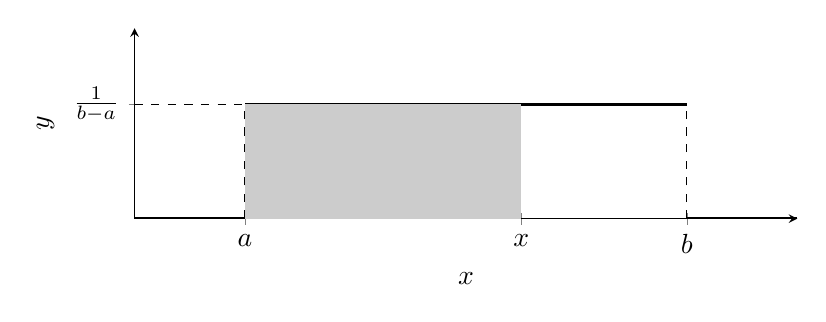
\begin{tikzpicture}

        \definecolor{siva}{rgb}{0.8, 0.8, 0.8}

        \begin{axis}[
            axis lines = left,
            xlabel = $x$,
            ylabel = {$y$},
            domain=-3:3,
            samples=100,
            height=4cm,
            width=10cm,
            xmin=-3, xmax=3,
            ymin=0, ymax=0.5,
            ytick={0.3},
            xtick={-2, 0.5, 2},
            yticklabels={$\frac{1}{b-a}$},
            xticklabels={$a$, $x$, $b$},
            yticklabel style={xshift=0cm}
        ]
        
        \draw[line width=1pt] (-3, 0) -- (-2, 0);
        \draw[line width=1pt] (-2, 0.3) -- (2, 0.3);
        \draw[line width=1pt] (2, 0) -- (3, 0);
    
        \draw[dashed] (-2, 0) -- (-2, 0.3);
        \draw[dashed] (2, 0) -- (2, 0.3);
        \draw[dashed] (-3, 0.3) -- (2, 0.3);
    
        \fill[siva] (-2,0) rectangle (0.5,0.3);
    
        \end{axis}
    \end{tikzpicture}
    $$
    F(x)=\int_{-\infty}^x p(t) \, d t= 
    \begin{cases}
        0, & \text{ če } x \leq a \\
        \frac{x-a}{b-a}, & \text{ če } a \leq x \leq b \\
        1, & \text{ če } x \geq b
    \end{cases}
    $$
    \item \emph{Normalna} ali \emph{Gaussova porazdelitev} $\operatorname{N}(\mu, \sigma)$, $(\mu \in \mathbb{R}, \sigma>0)$:
    $$
    p(x)=\frac{1}{\sigma \sqrt{2 \pi}} e^{-\frac{1}{2}\left(\frac{x-\mu}{\sigma}\right)^2}
    $$

    \begin{tikzpicture}
        \begin{axis}[
            axis lines = left,
            xlabel = $x$,
            ylabel = {$y$},
            domain=-3:3,
            samples=100,
            height=4cm,
            width=10cm,
            xmin=-3, xmax=3,
            ymin=0, ymax=0.5,
            xtick={0},
            xticklabels={$\mu$},
            yticklabels={}
        ]
        
        \addplot [black, thick] {1/(sqrt(2*pi))*exp(-(x^2/2)};
        \draw[dashed] (0, 0) -- (0, 0.3989);

        \end{axis}
    \end{tikzpicture}

    Če je $\sigma$ majhen: \hspace{5cm} Če je $\sigma$ velik:
    \begin{figure}[h]
        \begin{minipage}{0.45\textwidth}
            \centering
            \begin{tikzpicture}
                \begin{axis}[
                    axis lines = left,
                    xlabel = $x$,
                    ylabel = {$y$},
                    domain=-3:3,
                    samples=100,
                    height=4cm,
                    width=7cm,
                    xmin=-3, xmax=3,
                    ymin=0, ymax=1,
                    xtick={0},
                    xticklabels={$\mu$},
                    yticklabels={}
                ]
                
                \addplot [black, thick] {1/(sqrt(2*pi*0.22))*exp(-(x^2/(2*0.05))};
                \draw[dashed] (0, 0) -- (0, 0.8505);
        
                \end{axis}
            \end{tikzpicture}
        \end{minipage}
        \hfill
        \begin{minipage}{0.45\textwidth}
            \centering
            \begin{tikzpicture}
                \begin{axis}[
                    axis lines = left,
                    xlabel = $x$,
                    ylabel = {$y$},
                    domain=-3:3,
                    samples=100,
                    height=4cm,
                    width=7cm,
                    xmin=-3, xmax=3,
                    ymin=0, ymax=0.5,
                    xtick={0},
                    xticklabels={$\mu$},
                    yticklabels={}
                ]
                
                \addplot [black, thick] {1/(sqrt(2*pi*4))*exp(-(x^2/4)};
                \draw[dashed] (0, 0) -- (0, 0.1995);
        
                \end{axis}
            \end{tikzpicture}
        \end{minipage}
    \end{figure}

    $$
    F(x)=\frac{1}{\sigma \sqrt{2 \pi}} \int_{-\infty}^x e^{-\frac{1}{2}\left(\frac{x-\mu}{\sigma}\right)^2} \, d t \stackrel{\star}{=} \frac{1}{\sqrt{2 \pi}} \int_{-\infty}^{\frac{x-\mu}{\sigma}} e^{-\frac{1}{2}s^2} \, ds = \frac{1}{2}+\phi\left(\frac{x-\mu}{\sigma}\right)
    $$

    Kjer smo v enakosti $\star$ uvedli novo spremenljivko $s=\frac{t-\mu}{\sigma}$.
    
    \hspace{20pt} Tukaj je: $$\phi(x)=\frac{1}{\sqrt{2 \pi}} \int_0^x e^{2 \pi t^2} \, d t$$ \s

    $N(0,1)$: standardna normalna porazdelitev:
    $$
    p(x)=\frac{1}{\sqrt{2 \pi}} e^{-\frac{x^2}{2}}
    $$
    
    Laplaceova formula: za velike $n$ je:
    $$
    \operatorname{Bin}(n,p) \approx \operatorname{N}(np, \sqrt{npq})
    $$
    \begin{zgled}
        Sistolični krvni tlak je an populciji približno normalno porazdeljen: \s
        
        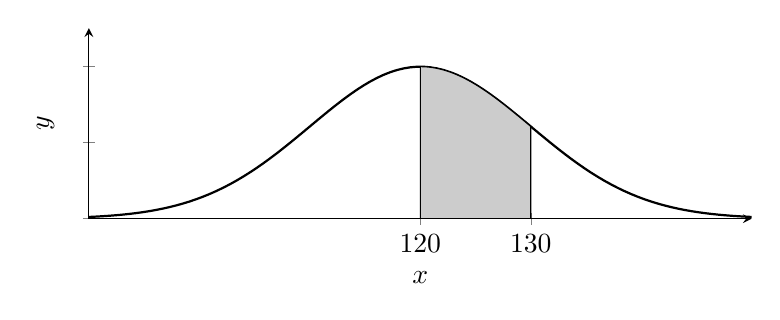
\begin{tikzpicture}

            \definecolor{siva}{rgb}{0.8, 0.8, 0.8}

            \begin{axis}[
                axis lines = left,
                xlabel = $x$,
                ylabel = {$y$},
                domain=-3:3,
                samples=100,
                height=4cm,
                width=10cm,
                xmin=-3, xmax=3,
                ymin=0, ymax=0.5,
                xtick={0, 1},
                xticklabels={120, 130},
                yticklabels={}
            ]
            
            \addplot [black, thick] {1/(sqrt(2*pi))*exp(-(x^2/2)};
            \addplot [fill=siva, domain=0:1] {1/(sqrt(2*pi))*exp(-(x^2/2)} \closedcycle;
            \draw[dashed] (0, 0) -- (0, 0.3989);
            \draw[dashed] (1, 0) -- (1, 0.2420);
        
            \end{axis}
        \end{tikzpicture}

        delež ljudi, ki imajo tlak med $120$ in $130 \operatorname{mm\ Hg}$.
    \end{zgled}

    \item \emph{Eksponenta porazdelitev} $\operatorname{Exp}(\lambda)$, $\lambda > 0$:
    $$
    p(x)= \begin{cases}\lambda e^{-\lambda x}, & \text { če } x \geq 0 \\ 0, & \text { sicer }\end{cases}
    $$

    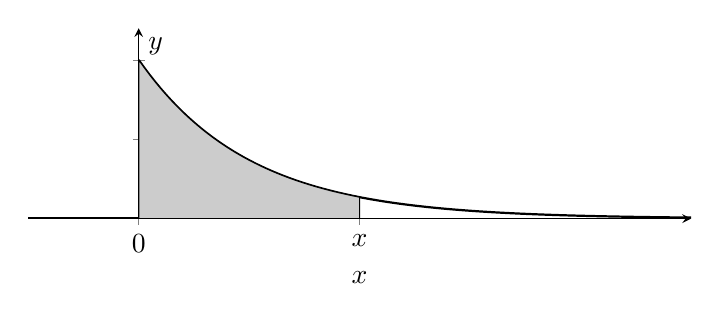
\begin{tikzpicture}

        \definecolor{siva}{rgb}{0.8, 0.8, 0.8}

        \begin{axis}[
            axis lines = left,
            xlabel = $x$,
            ylabel = {$y$},
            domain=0:5,
            samples=100,
            height=4cm,
            width=10cm,
            xmin=-1, xmax=5,
            ymin=0, ymax=1.2,
            axis y line=middle,
            xtick={0, 2},
            xticklabels={0, $x$},
            yticklabels={}
        ]
        
        \addplot [black, thick] {e^(-x)};
        \addplot [fill=siva, domain=0:2] {e^(-x)} \closedcycle;

        \draw[line width=1pt] (-1, 0) -- (0, 0);
        \draw[dashed] (0, 0) -- (0, 1);
        \draw[dashed] (2, 0) -- (2, 0.1353);
    
        \end{axis}
    \end{tikzpicture}

    $$
    F(x)= \begin{cases}1-e^{-\lambda x}, & \text { če } x \geq 0 \\ 0, & \text { sicer }\end{cases}
    $$

    \begin{tikzpicture}

        \definecolor{siva}{rgb}{0.8, 0.8, 0.8}

        \begin{axis}[
            axis lines = left,
            xlabel = $x$,
            ylabel = {$y$},
            domain=0:5,
            samples=100,
            height=4cm,
            width=10cm,
            xmin=-1, xmax=5,
            ymin=0, ymax=1.2,
            axis y line=middle,
            xtick={0, 2},
            ytick={1},
            xticklabels={0, $x$},
            yticklabels={1}
        ]
        
        \addplot [black, thick] {1-e^(-x)};

        \draw[line width=1pt] (-1, 0) -- (0, 0);
        \draw (2, 0) -- (2, 1-0.1353);
        \draw[dashed] (0, 1) -- (5, 1);
    
        \end{axis}
    \end{tikzpicture}

    \begin{zgled}
        Radioaktivni razpad - potreben čas, da se nekaj zgodi. 
    \end{zgled}

    \item \emph{Cauchyjeva porazdelitev}:
    $$
    p(x)=\frac{1}{\pi \left(1+x^2\right)}, \quad \text{za } x \in \mathbb{R}
    $$
    \begin{tikzpicture}
        \begin{axis}[
            axis lines = left,
            xlabel = $x$,
            ylabel = {$y$},
            domain=-3:3,
            samples=100,
            height=4cm,
            width=10cm,
            xmin=-3, xmax=3,
            ymin=0, ymax=0.5,
            ytick={0.3183},
            yticklabels={$\frac{1}{\pi}$},
            xticklabels={}
            enlargelimits=0.05,
            axis y line=middle,
            yticklabel style={xshift=-2cm}
        ]
        
        \addplot [black, thick] {1/(3.1415 * (1 + x^2))};
        \draw[dashed] (0, 0.3183) -- (-1.58, 0.3183);

        \end{axis}
    \end{tikzpicture}

    $$
    F(x)=\int_{-\infty}^x \frac{d t}{\pi\left(1+t^2\right)}=\left.\frac{1}{\pi} \operatorname{arctg} t\right|_{-\infty} ^x=\frac{1}{\pi} \operatorname{arctg} x+\frac{1}{2}
    $$
\end{enumerate}
\s
\begin{zgled}
    Primer slučajne spremenljivke, ki ni niti diskretno niti zvezno porazdeljena. 

    \n Vržemo pošten kovanec. Če pade grb, postavimo $X=1$; če pade cifra, naj bo $X$ slučajno izbrano število na intervalu $[0,2]$. \vspace{2pt}
    
    \n Izračunajmo $F(x)=P(X \leq x)$:
    
    1) Če je $x<0$, je $F(x) = 0$. Če je $x>2$, je $F(x) = 1$.

    2) Vzemimo, da je $0 \leq x \leq 2$. Potem je:
    $$
    F(x) = P(\text{grb}) P(X\leq x \mid \text{grb}) + P(\text{cifra}) P(X\leq x \mid \text{cifra})
    $$

    \qquad Če je $x<1$, je $F(x)=\frac{1}{2} \cdot \frac{x}{2}=\frac{x}{4}$.

    \qquad Če je $x \geq 1$, je $F(x)=\frac{1}{2}+\frac{1}{2} \cdot \frac{x}{2}=\frac{1}{2}+\frac{x}{4}$.

    \n Torej je: 
    $$
    F(x)=
    \begin{cases}
        0, & \text{ če } x<0 \\
        \frac{x}{4}, & \text{ če } 0 \leq x<1 \\
        \frac{1}{2}+\frac{x}{4}, & \text{ če } 1 \leq x \leq 2 \\
        1, & \text{ če } x>2
    \end{cases}
    $$

    \begin{tikzpicture}
        \begin{axis}[
            axis lines = left,
            xlabel = $x$,
            ylabel = {$y$},
            domain=-3:3,
            samples=100,
            height=4cm,
            width=10cm,
            xmin=-1, xmax=5,
            ymin=0, ymax=1.3,
            ytick={0.25, 0.75, 1.1},
            xtick={0, 2, 4},
            yticklabels={$\frac{1}{4}$, $\frac{3}{4}$, 1},
            xticklabels={0, 1, 2},
            axis y line=middle
        ]
        
        \draw[->, line width=1pt] (-1,0) -- (0,0);
        \draw[->, line width=1pt] (0,0) -- (2,0.25);
        \draw[->, line width=1pt] (2,0.75) -- (4,1);
        \draw[->, line width=1pt] (4,1) -- (6,1);
        \draw[dashed] (0, 1) -- (4, 1);
        \draw[dashed] (4, 0) -- (4, 1);

        \end{axis}
    \end{tikzpicture}

    \n Ker $F$ ni zvezna, $X$ ni zvezno porazdeljena. Ker $F$ ni odsekoma konstantna, $X$ ni diskretno porazdeljena. 
\end{zgled}

\chapter{Slučajni vektorji in neodvisnost}

\begin{definicija}
    \emph{Slučajni vektor} je $n$-terica slučajnih spremenljivk $X=\left(X_1, \ldots, X_n\right)$, to je preslikava $X:\Omega \to \mathbb{R}^n$ z lastnostjo, da je množica: 
    $$
    \left(X_1 \leq x_1, \ldots, X_n \leq x_n\right):=\left\{\omega \in \Omega: X_1(\omega) \leq x_1,\ldots, X_n(\omega) \leq x_n\right\}
    $$

    dogodek, za vsako $n$-terico $x=\left(x_1, x_2, \ldots, x_n\right) \in \mathbb{R}^n$.
\end{definicija}

\begin{definicija}
    \emph{Porazdelitvena funkcija} $F_X: \mathbb{R}^n \to \mathbb{R}$ je definirana s:
    $$
    F_X(x) \equiv F_{\left(X_{1, \ldots}, X_n\right)}\left(x_1, \ldots, x_n\right)=P\left(X_1 \leq x_1, \ldots, X_n \leq x_n\right)
    $$
\end{definicija}

\n Za vsak $x \in \mathbb{R}^n$ je $F(x) \in[0, 1]$.

\n Glede na vsako spremenljivko je $F$ naraščujoča in z desne zvezna:
$$
\begin{aligned}
    &\lim _{x_i \to \infty \, \forall i} F\left(x_1, \ldots, x_n\right)=1 \\
    &\lim _{x_i \rightarrow-\infty} F\left(x_1, \ldots, x_n\right)=0
\end{aligned}
$$

\n Če pošljemo proti $\infty$ samo nekatere spremenljivke, dobimo porazdelitvene funkcije podvektorjev, na primer:
$$
\begin{aligned}
    &\lim _{x_n \to \infty} F_{\left(X_1, \ldots, X_{n}\right)}\left(x_1, \dots , x_n\right)=F_{\left(X_1, \ldots, X_{n-1}\right)}\left(x_1, x_2, \ldots, x_{n-1}\right) \\
    &\lim _{\substack{x_2 \to \infty \\ \vdots \\x_n \to \infty}} F_{\left(X_1, \ldots, X_{n}\right)}\left(x_1, x_2, \ldots, x_n\right)=F_{X_1}\left(x_1\right)
\end{aligned}
$$

Take porazdelitvene funkcije za $X_1$ imenujemo tudi, \emph{robne} (marginalne) \emph{porazdelitve.}

\n Oglejmo si dvorazsežen primer:
$$
\begin{aligned}
    (X, Y): \Omega & \to \mathbb{R}^2 \\
    \omega & \mapsto(X(\omega), Y(\omega))
    \end{aligned}
$$

Porazdelitvena funkcija je: 
$$
F_{(X, Y)}(x, y)=P(X \leq x, Y \leq y)
$$

Robni porazdelitvi sta: 
$$
\begin{aligned}
    &F_X(x)=\lim _{y \rightarrow \infty} F_{(X, Y)}{(x, y)} \\
    &F_Y(y)=\lim _{x \rightarrow \infty} F_{(X,Y)}(x, y)
\end{aligned}
$$

\s

\n Izpeljimo analog formule $P\left(x_1<X \leq x_2\right)=F\left(x_2\right)-F\left(x_1\right)$, t.j. izračunajmo verjetnost:
$$
P(a<X \leq b, c<y \leq d)
$$

s pomočjo porazdelitvene funkcije $F_{(X, Y)}=F$.

\n Najprej si oglejmo:
$$
\begin{aligned}
    P(a<X \leq b, Y \leq d)&=P\left((X \leq b, Y \leq d) \setminus (X \leq a, Y \leq d)\right) \\
    &=P(X \leq b, Y \leq d)-P(X \leq a, Y \leq d) \\
    &=F(b, d)-F(a, d)
\end{aligned}
$$

\n V splošnem primeru: 
$$
\begin{aligned}
    P(a<X \leq b, c<Y \leq d)&=P(a<X \leq b, Y \leq d) - P(a<X \leq b, Y \leq c) \\
    &=F(b, d)-F(a, d) - (F(b, c)-F(a, c)) \\
    &=F(b, d)-F(a, d)-F(b, c)+F(a, c)
\end{aligned}
$$

\n Omejimo se na diskretne porazdelitve. 

Zaloga vrednosti slučajnih vektorjev $X=\left(X_1, \ldots, X_n\right)$ je največ števna množica v $\mathbb{R}^n$. Omejimo se na $n=2$: $(X, Y): \Omega \to \mathbb{R}^2$ z največ števno zalogo vrednosti. 

Naj bo $\left\{x_1, x_2, \ldots\right\}$ zaloga vrednosti za $X$, $\left\{y_1, y_2, \ldots\right\}$ pa zaloga vrednosti za $Y$. Očitno je zaloga vrednosti $(X,Y)$ vsbovana v množica:
$$
\left\{\left(x_i, y_j\right): i=1,2, \ldots, j=1,2, \ldots\right\}
$$

\n Verjetnostna funkcija:
$$
p_{i j}:=P\left(X=x_i, Y=y_j\right) \quad \text{za} \quad i=1, 2, \ldots \text{ in } j=1, 2, \ldots
$$
$$
\begin{array}{c|cccc|c}
    X\setminus Y & y_1 & y_2 & \cdots & y_n & X \\
    \hline x_1 & p_{11} & p_{12} & \cdots & p_{1 n} & p_1 \\
    x_2 & p_{21} & p_{22} & \cdots & p_{2 n} & p_2 \\
    \vdots & \vdots & \vdots & \ddots & \vdots & \vdots \\
    x_m & p_{m 1} & p_{m 2} & \cdots & p_{m n} & p_m \\
    \hline Y & q_1 & q_2 & \cdots & q_n & 1
    \end{array}
$$

$$
\begin{aligned}
    &p_i=P\left(X=x_i\right)=\sum_j P\left(X=x_i, Y=y_j \right)=\sum_j p_{ij} \\
    &q_j=P\left(Y=y_j\right)=\sum_i p_{ij}
\end{aligned}
$$

\begin{zgled}
    Met dveh kock: 
    $$
    \begin{array}{c|cccc|c}
        X \setminus Y & 1 & 2 & \ldots & 6 & X \\
        \hline 1 & \frac{1}{36} & \frac{1}{36} & \cdots & \frac{1}{36} & \frac{1}{6}\\
        2 & \frac{1}{36} & \frac{1}{36} & \cdots & \frac{1}{36} & \frac{1}{6}\\
        \vdots & \vdots & \vdots & \ddots & \vdots & \vdots \\
        6 & \frac{1}{36} & \frac{1}{36} & \cdots & \frac{1}{36} & \frac{1}{6} \\
        \hline Y & \frac{1}{6} & \frac{1}{6} & \cdots & \frac{1}{6} & 1
    \end{array}
    $$
\end{zgled}

\n Slučajne spremenljivke $X_1, X_2, \ldots, X_n$ so \emph{neodvisne}, če velja: 
$$
F_{\left(X_1, X_2, \ldots, X_n\right)}\left(x_1, x_2, \ldots, x_n\right)=F_{X_1}\left(x_n\right) \cdot F_{X_2}\left(x_2\right) \cdots F_{x_n}\left(x_n\right)
$$

za vse $\left(x_2, x_2, \ldots x_n\right) \in \mathbb{R}^n$, torej dogodki $\left(X_1 \leq x_1\right),\left(X_2 \leq x_2\right), \ldots,\left(X_n \leq x_n\right)$ so neodvisni.

\begin{trditev}
    Naj bo $(X,Y)$ diskreten slučajni vektor, $p_{i j}=P\left(X=x_i, Y=y_j\right), p_i=P\left(x=x_i\right), q_j=P\left(Y=y_j\right)$ za $i=1, 2, \ldots$, $j=1, 2, \ldots$

    Potem sta $X$ in $Y$ neodvisni slučajni spremenljivki $\iff$ $p_{i j}=p_i \cdot q_j \quad \forall i, \forall j$. 
\end{trditev}

\begin{proof}
    $(\implies)$:
    \begin{flalign*}
        p_{i j}&=\lim _{h \to 0+} P\left(x_i-h<X \leq x_i, y_j-h< Y \leq y_j\right) \\
        &=\lim _{h \to 0}\left(F\left(x_i, y_j\right)-F\left(x_i-h, y_j\right)-F\left(x_i, y_j-h\right) +F\left(x_i-h, y_j-h\right)\right) \\
        &=\lim _{h \to 0}\left(F_X\left(x_i\right) F_Y\left(y_j\right)-F_X\left(x_i-h\right) F_Y\left(y_j\right)-F_X\left(x_i\right) F_Y\left(y_j-h\right) \right. + \tag{$\star$} \\
        & \hspace{9cm} +\left. F_x\left(x_i-h\right) F_y\left(y_j-h\right)\right) \\
        &=\lim_{h \to 0}\left(F_X\left(x_i\right)-F_X\left(x_i-h\right)\right) \cdot\left(F_Y\left(y_j\right)-F_Y\left(y_j-h\right)\right) \\
        &=P\left(X=x_i\right) \cdot P\left(Y=y_j\right) \\
        &=p_i q_j
    \end{flalign*}
    Kjer smo v vrstici $(\star)$ uporabili neodvisnost. \s

    $(\impliedby)$:
    \begin{flalign*}
        \quad F_{(X, Y)}(x, y)&=\sum_{\left\{i,j: x_i \leq x_1,y_j \leq y\right\}} p_{i j} & \\
        &=\sum_{\left\{i,j: x_i \leq x,y_j \leq y\right\}} p_i p_j & \\
        &=\left(\sum_{\{i: x_i \leq x\}} p_i\right)\left(\sum_{\{j: y_j \leq y\}} q_j\right) & \\
        &=P(X \leq x) P(Y \leq y) & \\
        &=F_X(x)  F_Y(y) &
    \end{flalign*}
\end{proof}

\chapter[Matematično upanja oz. pričakovana vrednost]{Matematično upanja oz.\\pričakovana vrednost}

\n Za končno slučajno spremenljivko 
    $X:\left(\begin{array}{llll}
    x_1 & x_2 & \cdots & x_n \\
    p_1 & p_2 & \cdots & p_n
    \end{array}\right)$
je \emph{matematično upanje} definirano kot: 
$$
E(x):=\sum_{k=1}^n x_k p_k
$$

Tako je v primeru $p_1=p_2=\ldots=p_n=\frac{1}{n}$ matematično upanje enako povprečni vrednosti: $E(x)=\frac{x_n+x_2+\cdots+x_n}{n}$. 

\n Naj ima sedaj $X$ neskončno zalogo vrednosti. Če je $X$ diskretna slučajna spremenljivka, s $p_k=P\left(X=x_k\right)$ za $k \in \mathbb{N}$, potem ima $X$ matematično upanje, če je: 
$$
\sum_{k=1}^{\infty}\left|x_k\right| p_k<\infty
$$

Tedaj je \emph{matematično upanje} definirano kot vsota vrste: 
$$
E(x):=\sum_{k=1}^{\infty} x_k p_k
$$

\n Če je $X$ zvezna slučajna spremenljivka, z gostoto $p(x)$, ima $X$ matematično upanje, če je:
$$
\int_{-\infty}^{\infty}|x|  p(x) \, d x<\infty
$$

Tedaj je \emph{matematično upanje} definirano kot: 
$$
E(x)=\int_{-\infty}^{\infty} x \, p(x) \, d x
$$

\begin{zgled}
    ~
    
    \begin{enumerate}
        \item $X \sim \operatorname{Ber}(p), p >0$, $X:\left(\begin{array}{cc} 0 & 1 \\ q & p \end{array}\right)$:
        $$
        E(x)=0 \cdot q+1 \cdot p=p
        $$
        \item \emph{Izrojena} ali \emph{degenerirana} slučajna spremenljivka $\exists x_0 \in \mathbb{R}: P\left(X=x_0\right)=1$, t.j.: $X:\left(\begin{array}{c} x_0 \\ 1 \end{array}\right)$:
        $$
        E(x)=x_0 \cdot 1=x_0
        $$
        \item $X \sim \operatorname{Poi}(\lambda), \lambda >0$, $p_k=\frac{\lambda^k}{k !}  e^{-\lambda}$ in $x_k = k$, za $k=0, 1, 2, \ldots$:
        $$
        E(x)=\sum_{k=0}^{\infty} x_k \, p_k=\sum_{k=0}^{\infty} k \, \frac{\lambda^k}{k !}  e^{-\lambda}=e^{-\lambda} \lambda \sum_{k=1}^{\infty} \frac{\lambda^{k-1}}{(k-1) !} = e^{-\lambda} \lambda e^\lambda=\lambda
        $$
        \item Enakomerna zvezna porazdelitev na $[a, b]$:
        $$
        \begin{aligned}
            E(X)&=\int_{-\infty}^{\infty} x \, p(x) \, d x \\
            &=\int_a^b x \, \frac{1}{b-a} \, d x \\
            &=\frac{1}{b-a} \, \int_a^b x \,d x \\
            &=\left.\frac{1}{b-a} \frac{x^2}{2}\right|_a ^b \\
            &=\frac{b^2-a^2}{(b-a) 2} \\
            &=\frac{a+b}{2}
        \end{aligned}
        $$
        \item $X \sim \operatorname{N}(0,1)$, $p(x)=\frac{1}{\sqrt{2 \pi}} e^{-\frac{x^2}{2}}$:
        \begin{align*}
            \int_{-\infty}^{\infty}|x| e^{-\frac{x^2}{2}} \, d x&=2 \int_0^{\infty} x \, e^{-\frac{x^2}{2}} \, d x \\
            &=2 \int_0^{\infty} e^{-u} \, d u \tag{$\star$} \\
            &=\left.2 \left(-e^{-u}\right)\right|_0 ^{\infty}=2<\infty
        \end{align*}
        $\implies$ $X$ ima matematično upanje. V vrstici $(\star)$ smo uporabili per-partes.
        $$
        E(x)=\frac{1}{\sqrt{2 \pi}} \int_{-\infty}^{\infty} x \, e^{-\frac{x^2}{2}} \, d t \stackrel{\text{liha}}{=} 0
        $$
        \item Cauchyjeva porazdelitev, $p(x)=\frac{1}{\pi\left(1+x^2\right)}$:
        $$
        \int_{-\infty}^{\infty}|x| \frac{1}{\pi\left(1+x^2\right)} \, d x =\frac{2}{\pi} \int_0^{\infty} \frac{x}{1+x^2} \, d x = \left.\frac{1}{\pi} \ln \left(1+x^2\right)\right|_0 ^{\infty}=\infty
        $$
        $\implies$ $X$ nima matematičnega upanja.
        \item $1-\frac{1}{2}+\frac{1}{3}-\frac{1}{4}+\frac{1}{5}-\ldots$ pogojno konvergentna vrsta. Če vzamemo: 
        $$
        x_k p_k=\frac{(-1)^{k+1}}{k}, \quad \text{za} \quad k=1,2,\ldots
        $$
        $$
        p_k=2^{-k}=\frac{1}{2^k}, \quad \sum_{k=1}^{\infty} p_k=1, \quad x_k=\frac{(-1)^{k+1}}{k} 2^k
        $$
        $X$ nima matematičnega upanja, ker vrsta ne konvergira absolutno. 
    \end{enumerate}
\end{zgled}

\begin{trditev}
    Naj bo $f: \mathbb{R} \rightarrow \mathbb{R}$ funkcija: 
    \begin{enumerate}[label=(\alph*)]
        \item Če je 
            $X:\left(\begin{array}{cccc}
            x_1 & x_2 & x_3 & \cdots \\
            p_1 & p_2 & p_3 & \cdots
            \end{array}\right)$, potem je:
        $$
        E(f \circ X)=\sum_k f\left(x_k\right) p_k
        $$
        če matematično upanje obstaja, t.j. vrsta absolutno konvergira.
        \item Če je $X$ zvezno porazdeljena z gostoto $p(x)$, potem je: 
        $$
        E\left(f \circ X\right)=\int_{-\infty}^{\infty} f(x) p(x) \, d x
        $$
        če je integral absolutno konvergenten.
    \end{enumerate}
\end{trditev}

\begin{proof}(samo (a))
    $$
    f \circ X \equiv f(X):\left(\begin{array}{cccc}
        f\left(x_1\right) & f\left(x_2\right) & f\left(x_3\right) & \cdots \\
        p_1 & p_2 & p_3 & \cdots
        \end{array}\right)
    $$
    $$
    E(f \circ x)=\sum_h f\left(x_k\right) p_k
    $$
\end{proof}

\begin{posledica}
    Slučajna spremenljivka $X$ ima matematično upanje $\iff$ $|X|$ ima matematično upanje. Tedaj velja: 
    $$
    |E(X)| \leq E(|X|)
    $$
\end{posledica}
    
\begin{proof}
    $$
    |E(X)|=\left|\sum_k x_k  p_k \right| \leq \sum_k\left|x_k\right| p_k = E(|X|)
    $$
\end{proof}

\begin{posledica}
    Za $a \in \mathbb{R}$ in slučajno spremenljivko $X$ z matematičnim upanjem velja: 
    $$
    E(a \cdot x)=a \cdot E(x)
    $$

    Upanje je homogeno.
\end{posledica}

\begin{proof}
    Vzamemo: 
    $$
    f(x)=a \cdot x
    $$
\end{proof}

\n Podobno kot zadnjo trditev se dokaže:
\begin{trditev}
    Naj bo $f: \mathbb{R}^2 \to \mathbb{R}$ funkcija, $(X,Y)$ pa diskretno porazdeljen slučajni vektor: 
    $$
    p_{i j}=P\left(x=x_i, y=y_j\right), \quad \text{za} \quad i, j=1,2, \ldots
    $$
    Potem je $f(X, Y): \Omega \to \mathbb{R}$ slučajna spremenljivka in velja: 
    $$
    E(f(X, Y))=\sum_i \sum_j f\left(x_i, y_j\right)  p_{i j}
    $$

    če vrsta absolutno konvergira.
\end{trditev}

\begin{trditev}
    Če imata $X$ in $Y$ matematično upanje, ga ima tudi $X+Y$ in velja: 
    $$
    E(X+Y)=E(X)+E(Y)
    $$

    Upanje je aditivno. 
\end{trditev}

\begin{proof}
    $$
    \begin{aligned}
        E(X+Y)&=\sum_i \sum_j\left(x_i+y_j\right) p_{i j} \\
        &=\sum_i x_i \sum_j p_{i j}+\sum_j y_j \sum_i p_{i j} \\
        &=\sum_i x_i p_i+\sum_j y_j q_j \\
        &=E(X) + E(Y)
    \end{aligned}
    $$
\end{proof}

\begin{posledica}
    Za slučajne spremenljivke $X_1, X_2, \ldots, X_n$, ki imajo matematično upanje, velja: 
    $$
    E\left(a_1 X_1+a_2 X_2+\ldots+a_n X_n\right)=a_1 E\left(X_1\right)+a_2 E \left(X_2\right)+\cdots+a_n E\left(X_n\right)
    $$

    kjer so $a_1, a_2, \ldots, a_n \in \mathbb{R}$.
\end{posledica}

\begin{zgled}
    ~

    \begin{enumerate}
        \item Naj ima $X$ matematično upanje. Potem je: 
        $$
        E(X-E(X))=E(X)-E(\underbrace{E(X)}_{\text{konst.}})=E(X)-E(X)=0
        $$
        \item $X_k \sim \operatorname{Ber}(p)$, torej $X_k:\left(\begin{array}{cc}0 & 1 \\1-p & p\end{array}\right)$ za $k=1, 2, \ldots$. $X:=X_1+ \cdots +X_n$:
        $$
        E(X)=E\left(X_1\right)+\cdots+E\left(X_n\right)=n p
        $$
        Imejmo Bernoullijevo zaporedje neodvisnih ponovitev poskusa $A$, $P(A)=p$. $X_k:\left(\begin{array}{cc}0 & 1 \\1-p & p\end{array}\right)$; $(X_k=1)$, če se dogodek $A$ zgodi v $k$-ti ponovitvi poskusa. Potem je $X=X_1+\cdots+X_n$ frekvenca dogodka $A$ v $n$ ponovitvah. Tedaj je $X \sim \operatorname{Bin}(n,p)$.

        Torej je $E(X)=n p$. To se lahko vidi tudi direktno: 
        $$
        \begin{aligned}
            E(x)&=\sum_{k=0}^n k \binom{n}{k} p^k q^{n-k} \\
            &=\sum_{k=1}^n k  \frac{n}{k} \binom{n-1}{k-1} p^k q^{n-k} \\
            &=np \sum_{k=1}^n\binom{n-1}{k-1} p^{k-1} q^{n-k} \\
            &=n p (p+q)^{n-1} \\
            &= np
        \end{aligned}
        $$
    \end{enumerate}
\end{zgled}

\begin{zgled}
    $X \sim N(\mu, \sigma)$, $\mu \in \mathbb{R}, \sigma>0$:
    $$
    p(x)=\frac{1}{\sigma \sqrt{2 \pi}} e^{-\frac{1}{2}\left(\frac{x-\mu}{\sigma}\right)^2}
    $$

    Na vajah: $Y=\frac{X-\mu}{\sigma} \sim N(0,1)$. Ker je $E(Y) = 0$, je:
    $$
    E(x)=E(\sigma Y+\mu) = \sigma E(Y)+\mu=\mu
    $$
\end{zgled}

\begin{trditev}
    Če obstaja $E\left(X^2\right)$ in $E\left(Y^2\right)$, potem obstaja tudi $E(|X Y|)$ in velja: 
    $$
    E(|X Y|) \leq \sqrt{E\left(X^2\right) E\left(Y^2\right)}
    $$
    
    \n To je Cauchy-Schwarzova neenakost.

    Enakost velja $\iff$ 
    $$
    |Y|=\sqrt{\frac{E\left(Y^2\right)}{E\left(X^2\right)}} |X| \qquad \text{z verjetnostjo $1$.}
    $$ 
\end{trditev}

\begin{proof}
    Za poljubni nenegativni števili $u$ in $v$ velja: 
    $$
    u v \leq \frac{1}{2}\left(u^2+v^2\right) \qquad \left(\iff (u-v)^2 \geq 0 \right)
    $$
    Torej za nanegativni slučajni spremenljivki $U$ in $V$ velja:
    $$
    U V \leq \frac{1}{2}\left(U^2+V^2\right)
    $$

    kjer velja enačaj, le za $\omega \in \Omega$, v katerih je $U(\omega) = V(\omega)$.

    \n Če vstavimo $U=a|X|$ in $V=\frac{1}{a} |Y|$ za $a>0$, dobimo neenakost: 
    $$
    |X Y| \leq \frac{1}{2}\left(a^2 X^2+\frac{1}{a^2} Y^2\right)
    $$

    in zato je:
    $$
    E(|XY|) \leq \frac{1}{2}\left(a^2 E\left(X^2\right)+\frac{1}{a^2} E\left(Y^2\right)\right)
    $$  
    Če vstavimo $a^2=\sqrt{\frac{E\left(Y^2\right)}{E\left(X^2\right)}}$, je desna stran enaka: 
    $$
    \frac{1}{2}\left(\sqrt{\frac{E\left(Y^2\right)}{E\left(X^2\right)}}  E\left(X^2\right)+\sqrt{\frac{E\left(X^2\right)}{E\left(Y^2\right)}}  E\left(Y^2\right)\right) = \sqrt{E\left(X^2\right) E\left(Y^2\right)}
    $$

    torej je: 
    $$
    E(|X Y|) \leq \sqrt{E\left(X^2\right) E\left(Y^2\right)}
    $$
    Enačaj velja, če je $a |X|= \frac{1}{a}|Y|$, torej je:
    $$
    |Y|=a^2 |X|=\sqrt{\frac{E\left(Y^2\right)}{E\left(X^2\right)}} |X|
    $$
\end{proof}

\begin{posledica}
    Če obstaja $E\left(X^2\right)$, potem obstaja tudi $E(|X|)$ in velja:
    $$
    (E(|X|))^2 \leq E\left(X^2\right)
    $$
\end{posledica}

\begin{proof}
    $Y \equiv 1$
\end{proof}

\begin{trditev}
    Naj bosta $X$ in $Y$ neodvisni slučajni spremenljivki, ki imata matematično upanje. Potem obstaja tudi matematično upanje za $XY$ in velja: 
    $$
    E(X Y)=E(X) E(Y)
    $$
\end{trditev}

\begin{proof}(samo diskreten primer)
    $$
    E(XY)=\sum_i \sum_j x_i \, y_j \, p_{i j}
    $$
    
    po trditvi, kjer je $p_{ij}=P\left(X=x_i, Y=y_j\right)$.

    \n Zaradi neodvisnosti je $p_{i j}=p_i q_j$, kjer je $p_i=P\left(X=x_i\right)$ in $q_j=P\left(Y=y_j\right)$.

Torej je: 
    $$
    E(X Y)=\sum_i \sum_j x_i \, y_j \, p_i \, q_j = \left(\sum_i x_i \, p_i\right)\left(\sum_j y_j \, q_j\right)=E(X) E(Y)
    $$
\end{proof}

\n Če za $X$ in $Y$ velja $E(X Y)=E(X) E(Y)$, potem sta $X$ in $Y$ \emph{nekorelirani} slučajni spremenljivki. Sicer sta \emph{korelirani}.

Po trditvi iz neodvisnosti sledi nekoreliranost. Obrat ne velja.

\begin{zgled}
    $$
    U:\left(\begin{array}{ccc}
        0 & \frac{\pi}{2} & \pi \\
        \frac{1}{3} & \frac{1}{3} & \frac{1}{3}
        \end{array}\right)
    $$
    \begin{flalign*}
        &\qquad X = \sin U:\left(\begin{array}{ccc}
            0 & 1 & 0 \\
            \frac{1}{3} & \frac{1}{3} & \frac{1}{3}
            \end{array}\right)=\left(\begin{array}{cc}
            0 & 1 \\
            \frac{2}{3} & \frac{1}{3}
            \end{array}\right) & \\
        &\qquad Y=\cos U:\left(\begin{array}{ccc}
            -1 & 0 & 1 \\
            \frac{1}{3} & \frac{1}{3} & \frac{1}{3}
            \end{array}\right) &
    \end{flalign*}
    Velja:
    $$
    X Y=\sin U \cdot \cos U \equiv 0 \Rightarrow E(X Y)=0 
    $$
    $$
    E(X)=\frac{1}{3}, \quad E(Y)=-\frac{1}{3}+0+\frac{1}{3}=0
    $$
    $\quad \implies$ $X, Y$ sta nekorelirani.
    
    \n Poglejmo še neodvisnost:
    $$
    \begin{array}{c|ccc|c}
        X \setminus Y & -1 & 0 & 1 & \\
        \hline 0 & \frac{1}{3} & 0 & \frac{1}{3} & \frac{2}{3} \\
        1 & 0 & \frac{1}{3} & 0 & \frac{1}{3} \\
        \hline & \frac{1}{3} & \frac{1}{3} & \frac{1}{3} & 1
        \end{array}
    $$

    $X, Y$ sta odvisni slučajni spremenljivki.
\end{zgled}

\n \textbf{Domača naloga:} Za:
$$
X:\left(\begin{array}{cc}
    x_1 & x_2 \\
    p_1 & p_2
    \end{array}\right), \quad Y:\left(\begin{array}{cc}
    y_1 & y_2 \\
    q_1 & q_2
    \end{array}\right)
$$

Dokaži: $X$ in $Y$ sta nekorelirani $\iff$ neodvisni.

\chapter[Disperzija, kovarianca in korelacijski koeficient]{Disperzija, kovarianca in\\korelacijski koeficient}

Naj obstaja $E\left(X^2\right)$. \emph{Disperzija} oz. \emph{varianca} je definirana kot:
$$
D(X) \equiv \operatorname{Var}(X):=E\left((X-E(X))^2\right)
$$

$D(X)$ meri razpršenost okoli $E(X)$. 

\n Velja tudi: 
$$
\begin{aligned}
    E\left((X-E(X))^2\right)&=E\left(X^2-2 E(X) X+(E(X))^2\right) \\
    &=E\left(X^2\right)-2 E(X) E(X)+(E(X))^2 \\
    &=E\left(X^2\right)-(E(X))^2
\end{aligned}
$$

Zato je: 
$$
D(x)=E\left(X^2\right)-\left(E(X)\right)^2
$$

\n Lastnosti $D(X)$:

\begin{enumerate}
    \item $D(X) \geq 0 \text{ in } D(X) = 0 \iff P(X=E(X))=1$, t.j.: $X:\left(\begin{array}{c}E(X) \\ 1 \end{array}\right)$.
    \item $D(aX) = a^2 D(X)$ za $a \in \mathbb{R}$.
    \item Za vsak $a \in \mathbb{R}$ je $E\left((X-a)^2\right) \geq D(X)$. Enačaj velja $\iff$ $a=E(X)$.
    \begin{proof}
        $$
        \begin{aligned}
            E\left((X-a)^2\right)&=E\left(X^2-2 a X+a^2\right) \\
            &=E\left(X^2\right)-2 a  E(X)+a^2 \\
            &=(a-E(X))^2 - (E(X))^2+E\left(X^2\right) \\
            &=(a-E(X))^2+D(X) \geq D(X)
        \end{aligned}
        $$
    \end{proof}
\end{enumerate}

\n \emph{Standardna deviacija} oz. \emph{standardni odklon} je definirana kot: 
$$
\sigma(X):=\sqrt{D(X)}
$$

Zanjo velja $\sigma(a X)=\left|a\right| \sigma(X)$ za $a \in \mathbb{R}$. \s

\n Pregled nakaterih $E(X)$ in $D(X)$: 

\begin{enumerate}
    \item Enakomerna diskretna porazdelitev,
    $X:\left(\begin{array}{cccc}
        x_1 & x_2 & \cdots & x_n \\
        \frac{1}{n} & \frac{1}{n} & \cdots & \frac{1}{n}
    \end{array}\right)$:
    \begin{flalign*}
        & \quad E(X)=\frac{x_1+\cdots+x_n}{n}, \qquad D(X)=\frac{x_1^2+\cdots+x_n^2}{n}-\left(\frac{x_1+\cdots+x_n}{n}\right)^2&
    \end{flalign*}  
    \item Binomska porazdelitev, $\operatorname{Bin}(n, p)$:
    \begin{flalign*}
        & \quad E(X)=n p, \qquad D(X)=n  p q, \qquad \sigma(X)=\sqrt{n p q} &
    \end{flalign*}
    \item Poissonova porazdelitev, $\operatorname{Poi}(\lambda)$:
    \begin{flalign*}
        & \quad E(X)=D(X)=\lambda &
    \end{flalign*}
    \item Geometrijska porazdelitev, $\operatorname{geo}(p)$:
    \begin{flalign*}
        & \quad E(X)=\frac{1}{p}, \qquad D(x)=\frac{q}{p^2}, \quad \text{za} \quad q=1-p &
    \end{flalign*}
    \item Pascalova porazdelitev, $\operatorname{Pas}(m, p)$:
    \begin{flalign*}
        & \quad E(X)=\frac{m}{p}, \qquad D(X)=\frac{m q}{p}, \quad \text{za} \quad q=1-p &
    \end{flalign*}
    \item Enakomerna zvezna porazdelitev na $[a,b]$:
    \begin{flalign*}
        & \quad E(X)=\frac{a+b}{2}, \qquad D(X)=\frac{(b-a)^2}{12} &
    \end{flalign*}
    \item Normalna porazdelitev, $\operatorname{N}(\mu, \sigma)$:
    \begin{flalign*}
        & \quad E(X)=\mu, \qquad D(X)=\sigma^2, \qquad\sigma(x)=\sigma &
    \end{flalign*}
    \item Eksponenta porazdelitev, $\operatorname{Exp}(\lambda)$:
    \begin{flalign*}
        & \quad E(X)=\frac{1}{\lambda}, \qquad D(x)=\frac{1}{\lambda^2} &
    \end{flalign*}
\end{enumerate}

\begin{proof}(samo (4.))
    Velja: $p_k=p(X=k)=p q^{k-1}$ za $k=1, 2, 3, \ldots$
    $$
    \begin{aligned}
        \ E(X)&=\sum_{k=1}^{\infty} k p  q^{k-1} \\
        &=p \sum_{k=1}^{\infty} k q^{k-1} \\
        &=p \left(\sum_{k=0}^{\infty} q^k\right)^{\prime} \\
        &=p \left(\frac{1}{1-q}\right)^{\prime} \\
        &=p \frac{1}{(1-q)^2} \\
        &=\frac{1}{p}
    \end{aligned}
    $$
    \s
    $$
    \begin{aligned}
        E(X(X+1))&=\sum_{k=1}^{\infty} k(k+1) p q^{k-1} \\
        &=p \sum_{k=1}^{\infty}(k+1) k q^{k-1} \\
        &=p\left(\sum_{k=-1}^{\infty} q^{k+1}\right)^{\prime \prime} \\
        &=p \left(\frac{1}{1-q}\right)^{\prime \prime} \\
        &=p \left(\frac{1}{(1-q)^2}\right)^{\prime} \\
        &= p  \frac{2}{(1-q)^3} \\
        &= \frac{2}{p^2}
    \end{aligned}
    $$
    $$
    \implies D(X)=E(X(X+1))-E(X)-(E(X))^2 = \frac{2}{p^2}-\frac{1}{p}-\frac{1}{p^2}=\frac{1}{p^2}-\frac{1}{p}=\frac{q}{p^2}
    $$
\end{proof}

\begin{zgled}
    Met kocke. $X$ je število potrebnih metov, da pade prva šestica. $X \sim \operatorname{geo}(\frac{1}{6})$.
    $$
    E(X)=6, \qquad D(X)=\frac{\frac{5}{6}}{\frac{1}{36}}=30, \qquad \sigma(X)=\sqrt{30}
    $$
    \begin{tikzpicture}
        \begin{axis}[
            axis lines = left,
            xlabel = $x$,
            ylabel = {$y$},
            domain=-3:3,
            samples=100,
            height=4cm,
            width=10cm,
            xmin=-1, xmax=8,
            ymin=0, ymax=1.3,
            ytick={1},
            xtick={1, 2, 3, 4, 5, 6},
            yticklabels={$p$},
            xticklabels={1, 2, 3, 4, 5, 6},
            axis y line=middle
        ]
        
        \addplot[mark=*] coordinates {(1,1)};
        \addplot[mark=*] coordinates {(2,5/6)};
        \addplot[mark=*] coordinates {(3,5/6 * 5/6)};
        \addplot[mark=*] coordinates {(4,5/6 * 5/6 * 5/6)};
        \addplot[mark=*] coordinates {(5,5/6 * 5/6 * 5/6 * 5/6)};
        \addplot[mark=*] coordinates {(6,5/6 * 5/6 * 5/6 * 5/6 * 5/6)};
        \addplot[mark=*, mark size=1pt] coordinates {(7,5/6 * 5/6 * 5/6 * 5/6 * 5/6 * 5/6)};
        \addplot[mark=*, mark size=1pt] coordinates {(8,5/6 * 5/6 * 5/6 * 5/6 * 5/6 * 5/6 * 5/6)};
    
        \end{axis}
    \end{tikzpicture}

    $\quad p_1=p, \quad  p_2=p q, \quad p_3=p  q^2, \quad p_4 = p q^3, \quad\ldots$
\end{zgled}

\s

\n \emph{Kovarianca} slučajne spremenljivke $X$ in $Y$ se definirana kot: 
$$
\begin{aligned}
    K(Y, X) \equiv \operatorname{Cov}(X, Y)&:= E((X-E(X)) (Y-E(Y))) \\
    &=E(X Y-E(X) Y-X E(Y)+E(X) E(Y)) \\
    &=E(XY)-E(X)E(Y)-E(Y) E(X)+E(X) E(Y) \\
    &=E(XY)-E(X) E(Y)
\end{aligned}
$$

\n Lastnosti kovariance: 

\begin{enumerate}
    \item $K(X,X) = D(X)$
    \item $X$ in $Y$ sta nekorelirani $\iff$ $K(X,Y) = 0$
    \item $K$ je simetrična in bilinearna funkcija:
    \begin{flalign*}
        & \quad K(X, Y)=K(Y, X), \quad \text{za} \quad a, b \in \mathbb{R} & \\
        & \quad K(a X+b Y, Z)=a K(X, Z)+b K(Y, Z) & \\
    \end{flalign*}
    \item Kovarianca obstaja, če obstaja $D(X)$ in $D(Y)$. Tedaj velja:
    $$
    |K(X, Y)| \leq \sqrt{D(X) D(Y)}=\sigma(X) \sigma(Y),
    $$

    kar sledi iz Cauchy-Schwarzove neenakosti za $X-E(X)$ in $Y-E(Y)$. 
    
    Enakost velja $\iff$ $Y-E(Y)= \pm \frac{\sigma(Y)}{\sigma(X)} (X-E(X))$ z verjetnostjo $1$. 
    \item Če imata $X$ in $Y$ disperzijo, potem jo ima tudi $X+Y$ in velja: 
    $$
    D(X+Y)=D(X)+D(Y)+2 K(X, Y)
    $$
    
    Če sta $X$ in $Y$ nekorelirani, je potem: 
    $$
    D(X+Y)=D(X)+D(Y)
    $$ 
    \begin{proof}
        Sledi iz enakosti: 
        $$
        \begin{aligned}
            (X+Y-E(X+Y))^2&=\left((X-E(X))+(Y-E(Y))\right)^2 \\
            &= (X-E(X))^2+(Y-E(Y))^2 +\\
            &\hspace{4cm} +2(X-E(X)) (Y-E(Y))
        \end{aligned}
        $$
    \end{proof}
    \item Posplošitev zadnje lastnosti: 
    $$
    D\left(X_1+\cdots+X_n\right)=\sum_{k=1}^n D\left(X_k\right)+2 \sum_{i=1}^{n-1} \sum_{j=i+1}^n K\left(X_i, X_j\right)
    $$
    Posebej: če so $X_1, \ldots X_n$ paroma nekorelirane potem je: 
    $$
    D\left(X_1+\cdots+X_n\right)=D\left(X_1\right)+\cdots+D\left(X_n\right)
    $$
\end{enumerate}

\begin{zgled}
    Za $X \sim \operatorname{Bin}(n,p)$, je $X=X_1+\cdots+X_n$, kjer velja:
    $$
    X_k:\left(\begin{array}{cc} 0 & 1 \\ q & p \end{array}\right), \quad \text{oziroma} \quad X_k= \begin{cases}1, & \text { zgodi se $A$ v $k$-ti ponovitvi } \\ 0, & \text { sicer }\end{cases} 
    $$

    \n $X_1, \ldots X_n$ so neodvisne slučajne spremenljivke, zato je: 
    $$
    D\left(X_k\right)=E\left(X_k^2\right)-\left(E\left(X_k\right)\right)^2=p-p^2=p(1-p)=p q
    $$

    in potem: 
    $$
    D(X)=D\left(X_1+\cdots+X_n\right)=D\left(X_1\right)+\cdots+D\left(X_n\right)=n p q
    $$
\end{zgled}

\n \emph{Standardizacija} slučajne spremenljivke $X$ je slučajna spremenljivka: 
$$
X_s=\frac{X-E(X)}{\sigma(X)}
$$

Tedaj je $E\left(X_s\right)=0$ in $D\left(X_s\right)=1$, saj je: 
$$
D\left(X_s\right)=\frac{1}{\sigma(X)^2} \frac{D(X-E(X))}{D(X)}=1
$$

\begin{zgled}
    Na vajah boste pokazali: 
    $$
    X \sim \operatorname{N}(\mu, \sigma) \implies X_s = \frac{X - \mu}{\sigma} \sim \operatorname{N}(0,1)
    $$  
\end{zgled}

\n \emph{Korelacijski koeficient} slučajnih spremenljivk $X$ in $Y$ je: 
$$
r(X, Y)=\frac{K(X, Y)}{\sigma(X) \sigma(Y)}=\frac{E((X-E(X)) (Y-E(Y))}{\sigma(X) \sigma(Y)} = E(X_s Y_s)
$$

\n Lastnosti: 

\begin{enumerate}
    \item $r(X, Y)=0$ $\iff$ $X$ in $Y$ sta nekorelirani.
    \item $-1 \leq r(X, Y) \leq 1$
    \begin{proof}
        Sledi iz lastnosti (4) za $K$.  
    \end{proof}
    \item ~ \vspace{-31pt}
    $$
    \begin{aligned}
        &r(X, Y)=1 \iff Y=\frac{\sigma(Y)}{\sigma(X)} (X-E(X))+E(Y) \quad \text{z verjetnostjo $1$} \\
        &r(X, Y)=-1 \iff Y=-\frac{\sigma(Y)}{\sigma(X)} (X-E(X))+E(Y) \quad \text{z verjetnostjo $1$}
    \end{aligned}
    $$
\end{enumerate}

\begin{zgled}
    Vržemo 2 kocki. $X$ je število pik na prvi kocki in $Y$ število pik na drugi kocki. Zaradi neodvisnosti je $K(X,Y) = 0$. 

    Definiramo $Z=X+Y$. Izračunajmo $r(X,Z)$:
    \begin{flalign*}
        &\qquad E(X)=E(Y)=\frac{7}{2} & \\
        &\qquad E\left(X^2\right)=\frac{1}{6}(1+4+9+16+25+36)=\frac{91}{6} & 
    \end{flalign*}
    \begin{flalign*}
        &\qquad D(X)=E\left(X^2\right)-(E(X))^2=\frac{91}{6}-\frac{49}{4}=\frac{182-147}{12}=\frac{35}{12} & \\
        &\qquad K(X, Z)=K(X, X+Y)=K(X, X)+K(X, Y)=D(X)+0=\frac{35}{12} & \\
        &\qquad D(Z)=D(X)+D(Y)=2 \cdot \frac{35}{12}=\frac{35}{6}, \quad \text{ker sta $X$ in $Y$ neodvisni.} & \\
        &\qquad r(X, Z)=\frac{K(X, Z)}{\sqrt{D(X) D(Z)}}=\frac{\frac{35}{12}}{\sqrt{\frac{35}{12} \cdot \frac{35}{6}}}=\frac{1}{\sqrt{2}}=\frac{\sqrt{2}}{2} &
    \end{flalign*}
\end{zgled}

\chapter[Pogojna porazdelitev in pogojno matematično upanje]{Pogojna porazdelitev in\\pogojno matematično upanje}

\n Fiksirajmo dogodek $B$ s $P(B)>0$. \emph{Pogojna porazdelitvena funkcija} slučajne spremenljivke $X$ gleda na pogoj $B$ je: 
$$
F_X(x \mid B) = P(X \leq x \mid B)=\frac{P((X \leq x) \cap B)}{P(B)}
$$

Ima enake lastnosti kot porazdelitvena funkcija. 

\n Naj bo $(X,Y)$ diskreten slučajni vektor: 
$$
p_{i j}=P\left(X=x_i, Y=y_j\right), \quad B:=\left(Y=y_j\right), \quad P(B)=P\left(Y=y_j\right)=q_j
$$

\n Potem je pogojna porazdelitvena funkcija slučajne spremenljivke $X$ glede na $Y=y_j$: 
$$
\begin{aligned}
    F_X\left(x \mid y_j\right)&=F_X\left(x \mid Y=y_j\right) \\
    &=P\left(X \leq x \mid Y=y_j \right) \\
    &=\frac{1}{q_j} P\left((X \leq x) \cap\left(Y = y_j\right)\right) \\
    &=\frac{1}{q_j} \sum_{i : x_i \leq x} p_{i j}
\end{aligned}
$$

\n Vpeljemo \emph{pogojno verjetnostno funkcijo}:
$$
p_{i \mid j}=P\left(X=x_i \mid Y=y_j\right)=\frac{P\left(X=x_i, Y=y_j\right)}{P\left(Y=y_j\right)}=\frac{p_{i j}}{q_j}
$$

Tedaj je:
$$
F_X\left(x \mid Y=y_j\right)=\sum_{i: x_i \leq x} p_{i \mid j}
$$

\n \emph{Pogojno matematično upanje} slučajne spremenljivke $X$ gleda na $Y=y_j$ je matematično upanje te porazdelitve: 
$$
E\left(X \mid y_j\right) \equiv E\left(X \mid Y=y_j\right)=\sum_i x_i \, p_{i \mid j}=\frac{1}{q_j} \sum_i x_i \, p_{i j}
$$

Tako dobimo novo slučajno spremenljivko: 
$$
E(X \mid Y):\left(\begin{array}{ccc}
    E\left(X \mid y_1\right) & E\left(X \mid y_2\right) & \cdots \\
    q_1 & q_2 & \cdots
    \end{array}\right)
$$

\emph{Pogojno matematično upanje} slučajne spremenljivke $X$ glede na slučajno spremenjivko $Y$. 

\n Označimo $\varphi\left(y_j\right):=E\left(X \mid y_j\right)$ za vse $j$ in dobimo: 
$$
E(X \mid Y):=\varphi(Y):\left(\begin{array}{ccc}
    \varphi\left(y_1\right) & \varphi\left(y_2\right) & \cdots \\
    q_1 & q_2 & \cdots 
    \end{array}\right)
$$

$\varphi$ je \emph{regresijska funkcija}. 

\n Za $E(X,Y)$ velja zveza: 
$$
\begin{aligned}
    E(E(X \mid Y))&=\sum_j E\left(X \mid y_j\right) q_j \\
    &=\sum_j \sum_i x_i \, p_{i j} \\
    &=\sum_i x_i\left(\sum_j p_{i j}\right) \\
    &=\sum_i x_i \, p_i \\
    &=E(X)
\end{aligned}
$$

\n Vzemeimo, da sta $X$ in $Y$ neodvisni. Tedaj: 
$$
p_{i \mid j}=\frac{p_{i j}}{q_j}=p_i \implies E\left(X \mid y_j\right)=\sum_i x_i\, p_i=E(X)
$$

torej je $E(X \mid Y)$ izrojena slučajna spremenljivka.

\begin{zgled}
    Kokš znese $N$ jajc, kjer je $N \sim \operatorname{Poi}(\lambda)$. Iz vsakega jajca se zvali piščanec s verjetnostjo $p \in (0,1)$, neodvisno od drugih jajc. 

    Naj bo $K$ število piščancev. Določimo $E(K \mid N), E(K) \text { in } E(N \mid K)$.
    \begin{flalign*}
        &\qquad P(N=n)=\frac{\lambda^n}{n !} e^{-\lambda,} \quad \text{za} \quad n=0,1,2, \ldots & \\
        &\qquad P(K=k \mid N=h)=\binom{n}{k} p^{k} q^{n-k}, \quad q=1-p \quad \text{in za} \quad k=0,1,2, \ldots & \\
        &\qquad E(K \mid N=n)=E(\operatorname{Bin}(n, p))=n p=: \varphi(n) & \\
        &\qquad E(K \mid N)=p N=\varphi(N) & \\
        &\qquad E(K)=E(E(K \mid N))=E(p N)=p  E(N)=p  \lambda &
    \end{flalign*}
    Dokažimo, da je $K \sim \operatorname{Poi}(\lambda)$:
    \begin{flalign*}
        \qquad P(K=k)&=\sum_{n=k}^{\infty} P(K=k \mid N=n) P(N=n) & \\
        &=\sum_{n=k}^{\infty}\binom{n}{k} p^k \, q^{n-k} \, \frac{\lambda^n}{n !} e^{-\lambda} & \\
        &=e^{-\lambda} \frac{p^k}{k !} \lambda^k \sum_{n=k}^{\infty} \frac{q^{n-k} \, \lambda^{n-k}}{(n-k) !} & \\
        &=e^{-\lambda} \frac{(p \lambda)^k}{k !}  e^{q\lambda}=\frac{(p \lambda)^k}{k !} e^{-p \lambda} & 
    \end{flalign*}

    \begin{flalign*}
        \qquad P(N=n \mid K=k)&=\frac{P(N=n, K=k)}{P(K=k)} & \\
        &=\frac{P(K=k \mid N=n) P(N=n)}{P(K=k)} & \\
        &=\binom{n}{k} p^k \, q^{n-k} \frac{\lambda^n}{n !} e^{-\lambda}  \frac{k !}{(p \lambda)^k}  e^{p \lambda} & \\
        &=\frac{1}{(n-k) !} q^{n-k} \, \lambda^{n-k} e^{-q \lambda} & \\
        &=\frac{(q \lambda)^{n-k}}{(n-k) !} e^{-q \lambda} &
    \end{flalign*}
    
    za $n=k,k+1,k+2, \ldots$, kar je Poissonova porazdelitev, premaknjena za $k$ v desno: $k + \operatorname{Poi}(q \lambda)$. Zato je regresijska funkcija:
    $$
    \varphi(k)=E(N \mid K=k)=E(k+ \operatorname{Poi}(q \lambda))=k+q \lambda
    $$

    torej je: 
    $$
    E(N \mid K)=\varphi(K)=K+q \lambda
    $$

    Preizkus: 
    $$
    E(E(N \mid K))=E(K+q \lambda)=E(K)+q \lambda=p \lambda+q \lambda=\lambda = E(N)
    $$
\end{zgled}

\chapter{Rodovne funkcije}

\n Naj bo $X$ slučajna spremenljivka z vrednostmi v $\mathbb{N} \cup\{0\}$: 
$$
p_k=P(X=k), \quad \text{za} \quad k=0,1,2, \ldots, \quad p_k \geq 0, \quad \sum_{k=0}^{\infty} p_k=1
$$

\n \emph{Rodovna funkcija} slučajne spremenljivke $X$ je:
$$
G_X(s):=p_0+p_1 s+p_2 s^2+p_3 s^3+\cdots=\sum_{k=0}^{\infty} p_k s^k
$$

za vse $s \in \mathbb{R}$, za katere vrsta absolutno konvergira. 

\n Očitno je $G_X(0)=p_0$, $G_X(1)=\sum_{k=0}^{\infty} p_k=1$ in $G_X(s)=E\left( s^X\right)$, saj je: 
$$
s^X:\left(\begin{array}{ccccc}
    s^0 & s^1 & s^2 & s^3 & \cdots \\
    p_0 & p_1 & p_2 & p_3 & \cdots
    \end{array}\right)
$$

\n Za $s \in[-1,1]$ velja $\left|p_k \, s^k\right| \leq p_k$ in $\sum_{k=0}^{\infty} p_k=1$, zato vrsta $\sum_{k=0}^{\infty}\left|p_k \, s^k\right|$ konvergira. Torej je konvergenčni radij vrste vsaj $1$. 

\begin{zgled} ~

    \begin{enumerate}
        \item $X \sim \operatorname{geo}(p)$, $p_k=P(X=k)=p\, q^{k-1}$ za $k=1, 2, 3, \ldots$:
        $$
        G_X(s)=\sum_{k=1}^{\infty} p \, q^{k-1} s^k=p s \sum_{k=1}^{\infty}\left(qs\right)^{k-1} = p s \frac{1}{1-qs} = \frac{p s}{1-q s}
        $$

        za vse $s \in \mathbb{R}$, za katere je $|qs| < 1$, torej je konvergenčni radij $\frac{1}{q}$.
        \item $X \sim \operatorname{Poi}(\lambda)$, $p_k=p(X=k)=\frac{\lambda^k}{k !} e^{-\lambda}$ za $k=0,1,2, \ldots$:
        $$
        G_X(s)=\sum_{k=0}^{\infty} \frac{\lambda^k}{k !} e^{-\lambda} s^k=e^{-\lambda} \sum_{k=0}^{\infty}\frac{(\lambda s)^k}{k !}=e^{-\lambda} e^{\lambda s}=e^{\lambda(s-1)}
        $$

        za vse $s \in \mathbb{R}$.
    \end{enumerate}
\end{zgled}

\n Iz teorije Taylorjevih vrst dobimo \emph{izrek o enoličnosti}. 

\begin{izrek}
    Naj imata $X$ in $Y$ rodovni funkciji $G_X$ in $G_Y$. Potem za $s \in [-1, 1]$ velja:
    $$
    G_X(s)=G_Y(s) \iff P(X=k)=P(Y=k) \quad \text{za vse} \quad k=0, 1, 2, \ldots
    $$
\end{izrek}

\n Tedej velja: 
$$
P(X=k)=\frac{1}{k !} G_X^{(k)}(0)
$$ 

\s 

\n Velja: 
$$
G_X(s)=\sum_{k=0}^{\infty} p_k \, s^k, \quad  G_X^{\prime}(s)=\sum_{k=1}^{\infty} p_k \, k \,s^{k-1}
$$ 

za vse $s \in (-1, 1)$. Od koder sledi: 

$$
\lim _{s \uparrow 1} G_X^{\prime}(s)=\sum_{k=1}^{\infty} p_k \, k=E(X)
$$

\begin{izrek}
    Naj ima $X$ rodovno funkcijo $G_X$ in $n \in \mathbb{N}$. Potem je: 
    $$
    G_X^{(n)}(1-)=E(X(X-1)(X-2) \cdots(X-n+1))
    $$

    kjer je: $G_X^{(n)}(1-)=\lim_{s \uparrow 1} G_X^{(n)}(s)$
\end{izrek} 

\begin{proof}
    Za $s \in[0,1)$ je: 
    $$
    G_X^{(n)}(s)=\left(\sum_{k=0}^{\infty} p_k \, s^k\right)^{(n)}=\sum_{k=n}^{\infty} k(k-1) \cdots(k-n+1) s^{k-n} \, p_k
    $$
    Ko gre $s \uparrow 1$, z uporabo Abelove leme dobimo: 
    $$
    \lim_{s \uparrow 1} G_X^{(n)}(s)=\sum_{k=n}^{\infty} k(k-1) \cdots(k-n+1) \, p_k=E(X(X-1)(X-2) \cdots(X-n+1))
    $$
\end{proof}

\begin{posledica}
    \begin{flalign*}
        \qquad E(X)&=G_X^{\prime}(1-) & \\
        \qquad D(X)&=E(X(X-1))+E(X)-(E(X))^2  & \\
        &= G_X^{\prime \prime}(1-)+G_X^{\prime}(1-)-\left(G_X^{\prime}(1-)\right)^2 &
    \end{flalign*}
\end{posledica}

\begin{izrek}
    Naj bosta $X$ in $Y$ neodvisni slučajni spremenljivki z rodovnima funkcijama $G_X$ in $G_Y$. Potem je za $s \in [0,1]$: 
    $$
    G_{X+Y}(s)=G_X(s) \, G_Y(s)
    $$
\end{izrek}

\begin{proof}
    \begin{align*}
        G_{X+Y}(s)&=E\left(s^{X+Y}\right) \\
        &=E(s^X \cdot s^Y) \\
        &=E(s^X) \, E(s^Y) \tag{$\star$} \\
        &=G_X(s) \, G_Y(s)
    \end{align*}

    \n Enakost $(\star)$ velja, saj sta $s^X$ in $s^Y$ neodvisni slučajni spremenljivki.
\end{proof}

\n \textbf{Posplošitev:} Če je $S_n=X_1 + \cdots + X_n$ vsota neodvisnih slučajnih spremenljivk z vrednostmi v $\mathbb{N} \cup \{0\}$, potem je za $s \in [-1, 1]$: 
$$
G_{S_n}(s)=G_{X_1}(s)\, G_{X_2}(s) \cdots G_{X_n}(s)
$$

\n Posebej: če so $X_1, \ldots, X_n$ enako porazdeljene, potem je: 
$$
G_{S_n}(s)=\left(G_X(s)\right)^n
$$

\s

Kakšne so rodovne funkcije slučajne spremenljivke $S_N=X_1 + X_2 + \cdots + X_N$, kjer so $X_1, X_2, \ldots$ enako porazdeljene in $N$ slučajna spremenljivka z rodovno funkcijo $G_N$?

\begin{izrek}
    Naj bodo za vsak $n \in \mathbb{N}$ slučajne spremenljivke $N, X_1, X_2, \ldots, X_n$. Naj ima $N$ rodovno funkcijo $G_N$, $X_n$ pa rodovno funkcijo $G_X$ za vsak $n \in \mathbb{N}$. Potem ima slučajna spremenljivka $S=X_1+X_2+\cdots+X_N$ rodovno funkcijo: 
    $$
    G_S(s)=G_N\left(G_X(s)\right) \quad \text{za} \quad s \in [-1,1]
    $$
\end{izrek}

\begin{proof}
    Zaradi neodvisnosti imamo: 
    \begin{align*}
        P(S=k)&=\sum_{n=1}^{\infty} P(S=k, N=n) & \\
        &=\sum_{n=1}^{\infty} P\left(N=n, X_1+X_2+ \cdots +X_k=k\right) & \\
        &=\sum_{n=1}^{\infty} P(N=n) P\left(X_1+\cdots+X_n=k\right) & \tag{$\star$}
    \end{align*}
    
    Kjer vrstica $(\star)$ velja zaradi neodvisnosti. Zato je: 
    \begin{align*}
        G_S(s)&=\sum_{k=0}^{\infty} P(S=k) s^k & \\
        &=\sum_{n=1}^{\infty} P(N=N) \sum_{k=0}^{\infty} P\left(X_1+\cdots+X_n=k\right)  s^k & \\
        &=\sum_{n=1}^{\infty} P(N=n) \, G_{X_1+\cdots+X_n}\left(s\right) & \\
        &=\sum_{n=1}^{\infty} P(N=n) \left(G_X(s)\right)^n & \\
        &=G_N\left(G_X(s)\right)
    \end{align*}
\end{proof}

\begin{posledica}
    Waldova enakost: 
    $$
    E(S)=E(N) \, E(X)
    $$
\end{posledica}

\begin{proof}
    \begin{align*}
        E(S)&=G_S^{\prime}(1-) \\
        &=G_N^{\prime}(\underbrace{G_X(1-)}_{1-}) \, G_X^{\prime}(1-) \\
        &=E(N) \, E(X)
    \end{align*}
\end{proof}

\begin{zgled}[Kokoš, jajca, piščanci]
    $N$ jajc, $N \sim \operatorname{Poi}(\lambda)$, $\lambda > 0$. $K$ piščancev. Vpeljemo slučajne spremenljivke $X_1, X_2, \ldots$, kjer $(X_i=1)$, če se iz $i$-tega jajca izvali piščanec, sicer pa je $(X_i=0)$. Potem je: 
    $$
    X_i:\left(\begin{array}{cc}
        0 & 1 \\
        q & p
        \end{array}\right), \quad K = X_1 + X_2 + \cdots + X_N
    $$
    Ker je $G_N(s)=e^{\lambda (s-1)}$ in $G_X(s)=q+p  s$ je: 
    $$
    G_K(s)=G_N\left(G_X(s)\right)=e^{\lambda(q+p s-1)}=e^{\lambda p(s-1)}
    $$

    od koder sledi $K \sim \operatorname{Poi}(\lambda p)$.
\end{zgled}

\chapter[Višji momenti in vrstilne karakteristike]{Višji momenti in\\vrstilne karakteristike}

\n Naj bo $k \in \mathbb{N}$ in $a \in \mathbb{R}$. \emph{Moment reda $k$ glede na a} je:
$$
m_k(a)=E\left((X-a)^k\right)
$$

če obstaja. 

\n Za $a$ običajno vzamemo: 
\begin{enumerate}
    \item $a=0$: $z_k=m_k(0)=E\left(X^k\right)$; \emph{začetni moment}. 
    \item $a=E(X)$: $m_k=m_k(E(x))=E\left((X-E(X))^k\right)$; \emph{centralni moment reda $k$}.
\end{enumerate}

\n Očitno je $z_1=E(X)$ in $m_2=D(X)$. 

\begin{trditev}
    Če obstaja $m_n(a)$, potem obstaja tudi $m_k(a)$ za vsak $k<n$.
\end{trditev}

\begin{proof}
    \begin{align*}
        E\left(|X-a|^k\right)&=\sum_i\left|x_i-a\right|^k  p_i \\
        &=\sum_{i: | x_i-a | \leq 1} \underbrace{\left|x_i-a\right|^k}_{\leq 1} p_i+\sum_{i: | x_i-a |  >1}\left|x_i-a\right|^k p_i \\
        &\leq \sum_i p_i+\sum_i\left|x_i-a\right|^n p_i \\
        &=1+E\left(\left|X_i-a\right|^n\right) < \infty
    \end{align*}

    saj $m_n(a)$ obstaja.
\end{proof}

\begin{trditev}
    Če obstaja začetni moment $z_n$, potem obstaja tudi $m_n(a)$ za poljuben $a \in \mathbb{R}$.
\end{trditev}

\begin{proof}
    \begin{align*}
        E\left(|X-a|^n\right) &\leq E\left((|X|+|a|)^n\right) \\
        &=\sum_{n=0}^h \binom{n}{k}|a|^{n-k} \, E\left(|X|^k\right) < \infty
    \end{align*}

    po prejšnji trditvi.
\end{proof}

\n Velja: 
$$
m_n(a)=E\left((X-a)^n\right)=\sum_{k=0}^n\binom{n}{k}(-a)^{n-k} \, \underbrace{E\left(X^k\right)}_{z_k}
$$

Tako lahko centralne momente izračunamo z začetnimi momenti: 
$$
m_n=\sum_{k=0}^n \binom{n}{k} (-1)^{n-k} \, z_1^{n-k} \, z_k
$$

\s 

\n \emph{Asimetrija} slučajne spremenljivke $X$ je: 
$$
A(X):=E\left(X_s^3\right)=E\left(\left(\frac{X-E(X)}{\sigma(X)}\right)^3\right)=\frac{m_3}{m_2^{\frac{3}{2}}}
$$
 
Na primer: $A(N(\mu, \sigma))=0$, $A(\lambda X)=A(X)$ za $\lambda >0$.

\s 

\n \emph{Sploščenost (kurtozis)} slučajne spremenljivke $X$ je:
$$
K(X):=E\left(X_s^4\right)=E\left(\left(\frac{X-E(X)}{\sigma(X)}\right)^4\right)=\frac{m_4}{m_2^2}
$$

Na primer: $K(N(\mu, \sigma))=3$, $K(\lambda X)=K(X)$ za $\lambda > 0$.

\s \s

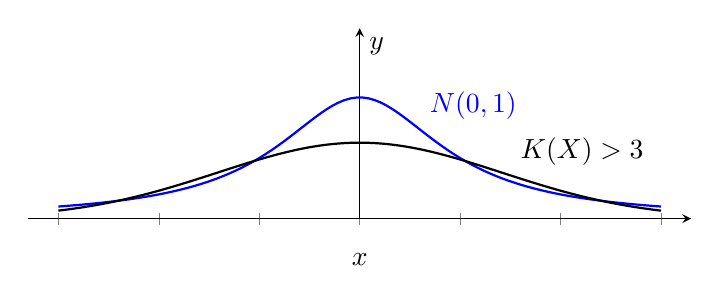
\begin{tikzpicture}
    \begin{axis}[
        axis lines = left,
        xlabel = $x$,
        ylabel = {$y$},
        domain=-3:3,
        samples=100,
        height=4cm,
        width=10cm,
        xmin=-3, xmax=3,
        ymin=0, ymax=0.5,
        ytick={0.3183},
        yticklabels={},
        xticklabels={},
        enlargelimits=0.05,
        axis y line=middle
    ]

    \addplot [blue, thick] {1/(3.1415 * (1 + x^2))} node[pos=0.6, above right] {$N(0,1)$};
    \addplot [black, thick] {1/(sqrt(2*pi*4))*exp(-(x^2/4))} node[pos=0.75, above right] {$K(X)>3$};
    
    \end{axis}
\end{tikzpicture}

Nekateri definirajo sploščenost kot $K(X) - 3$, torej je v primeru $N(\mu, \sigma)$ enaka 0. 

\s

Za razliko od momentov vedno obstajajo \emph{vrstilne karakteristike}.

\n \emph{Mediana} slučajne spremenljivke $X$ je vsaka vrednost $x \in \mathbb{R}$, za katero velja:
$$
P(X \leq x) \geq \frac{1}{2} \quad \text{in} \quad P(X \geq x) \geq\frac{1}{2}
$$

Ker je $P(X \geq x)=1-P(X<x)=1-F(x-)$, lahko pogoj za mediano zapišemo kot: 
$$
F(x-) \leq \frac{1}{2} \leq F(x)
$$

\n Če je $X$ zvezno porazdeljena, je pogoj enak $F(x) = \frac{1}{2}$.

\n Te vrednosti (lahko jih je več) označimo z $x_{\frac{1}{2}}$.

\begin{zgled} ~

    \begin{enumerate}
        \item $X:\left(\begin{array}{cc}
            0 & 1 \\
            \frac{1}{5} & \frac{4}{5}
            \end{array}\right)$, $x_{\frac{1}{2}} = 1$, $E(X) = \frac{4}{5}$:
        
        \begin{tikzpicture}
            \begin{axis}[
                axis lines = left,
                xlabel = $x$,
                ylabel = {$y$},
                domain=-3:3,
                samples=100,
                height=4cm,
                width=10cm,
                xmin=-1, xmax=5,
                ymin=0, ymax=1.3,
                ytick={0.2, 0.5, 1},
                xtick={0, 2},
                yticklabels={$\frac{1}{5}$, $\frac{1}{2}$, 1},
                xticklabels={0, 1},
                axis y line=middle
            ]
            
            \draw[->, line width=1pt] (-1,0) -- (0,0);
            \draw[->, line width=1pt] (0,0.2) -- (2,0.2);
            \draw[->, line width=1pt] (2,1) -- (6,1);
            \draw[dashed] (2, 0) -- (2, 1);
            \draw[dashed] (0, 0.5) -- (6, 0.5);
    
            \end{axis}
        \end{tikzpicture}
        \item $X:\left(\begin{array}{ccc}
            -1 & 0 & 1 \\
            \frac{1}{4} & \frac{1}{4} & \frac{1}{2}
            \end{array}\right)$, mediane so na $[0,1]$:

        \begin{tikzpicture}
            \begin{axis}[
                axis lines = left,
                xlabel = $x$,
                ylabel = {$y$},
                domain=-3:3,
                samples=100,
                height=4cm,
                width=10cm,
                xmin=-3, xmax=3,
                ymin=0, ymax=1.3,
                ytick={0.25, 0.5, 1},
                xtick={-2, 0, 2},
                yticklabels={$\frac{1}{4}$, $\frac{1}{2}$, 1},
                xticklabels={-1, 0, 1},
                axis y line=middle
            ]
            
            \draw[->, line width=1pt] (-4,0) -- (-2,0);
            \draw[->, line width=1pt] (-2,0.25) -- (0,0.25);
            \draw[->, line width=1pt] (0,0.5) -- (2,0.5);
            \draw[->, line width=1pt] (2,1) -- (4,1);
            \draw[dashed] (2, 0) -- (2, 1);
            \draw[dashed] (-2, 0) -- (-2, 0.25);
            \draw[dashed] (-6, 0.5) -- (6, 0.5);
    
            \end{axis}
        \end{tikzpicture}
        \item $X \sim N(\mu, \sigma)$, $x_{\frac{1}{2}} = \mu = E(X)$
        
        \begin{tikzpicture}
            \begin{axis}[
                axis lines = left,
                xlabel = $x$,
                ylabel = {$y$},
                domain=0:3,
                samples=100,
                height=4cm,
                width=10cm,
                xmin=0, xmax=3,
                ymin=0, ymax=0.5,
                xtick={1.5},
                xticklabels={$\mu$},
                yticklabels={},
                enlargelimits=0.05,
                axis y line=middle
            ]
            
            \addplot [black, thick] {1/(sqrt(2*pi*2))*exp(-((x-1.5))^2/0.5)};
            \draw[dashed] (1.5, 0) -- (1.5, 0.2820);

            \node at (1.30,0.15) {\small $\frac{1}{2}$};
            \node at (1.70,0.15) {\small $\frac{1}{2}$};
    
            \end{axis}
        \end{tikzpicture}
        \item ~
        
        \begin{tikzpicture}
            \begin{axis}[
                axis lines = left,
                xlabel = $x$,
                ylabel = {$y$},
                domain=-2:2,
                samples=100,
                height=4cm,
                width=10cm,
                xmin=-2, xmax=2,
                ymin=0, ymax=2,
                xtick={},
                xticklabels={},
                yticklabels={}
            ]
            
            \addplot [black, thick, domain=-1.5:-0.5] {(x-1.5)^2 * (x-0.5)^2 * (x+1.5)^2 * (x+0.5)^2};
            \addplot [black, thick, domain=0.5:1.5] {(x-1.5)^2 * (x-0.5)^2 * (x+1.5)^2 * (x+0.5)^2};
            \draw[line width=2pt] (-0.5,0) -- (0.5,0);
            \addplot[mark=*] coordinates {(-0.5,0)};
            \addplot[mark=*] coordinates {(0.5,0)};
    
            \node at (-1.1,0.4) {\small $\frac{1}{2}$};
            \node at (1.1,0.4) {\small $\frac{1}{2}$};
            \node at (0,0.3) {\small \text{mediane}};

            \end{axis}
        \end{tikzpicture}
    \end{enumerate}
\end{zgled}

\n \emph{Kvantil reda $p$} je vsaka vrednost $x_p$, za katero velja: 
$$
P\left(X \leq x_p\right) \geq p \quad \text{in} \quad P\left(X \geq x_p\right) \geq 1-p
$$

Oziroma ekvivalentno: 
$$
F\left(x_p-\right) \leq p \leq F\left(x_p\right), \quad  0<p<1
$$

\n Če je $X$ zvezno porazdeljena, je pogoj za kvantil: 
$$
F(x_p)=p \iff \int_{-\infty}^{x_p} p_X(t) \, d t=p
$$

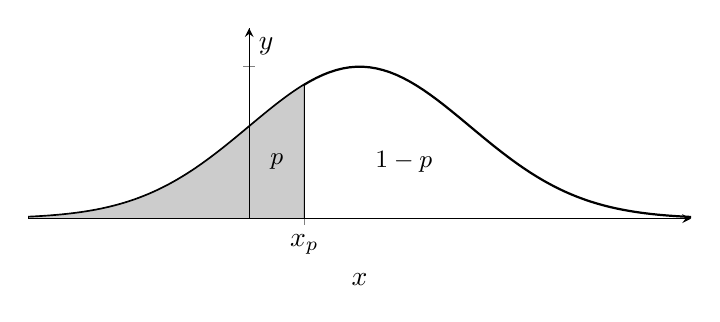
\begin{tikzpicture}

    \definecolor{siva}{rgb}{0.8, 0.8, 0.8}

    \begin{axis}[
        axis lines = left,
        xlabel = $x$,
        ylabel = {$y$},
        domain=-2:4,
        samples=100,
        height=4cm,
        width=10cm,
        xmin=-2, xmax=4,
        ymin=0, ymax=0.5,
        xtick={0.5},
        xticklabels={$x_p$},
        yticklabels={},
        axis y line=middle
    ]
    
    \addplot [black, thick] {1/(sqrt(2*pi))*exp(-((x-1)^2/2)};
    \addplot [fill=siva, domain=-2:0.5] {1/(sqrt(2*pi))*exp(-((x-1)^2/2)} \closedcycle;
    \draw (0,1) -- (0,0);
    
    \node at (0.25,0.15) {\small $p$};
    \node at (1.40,0.15) {\small $1-p$};

    \end{axis}
\end{tikzpicture}

\s

\n \emph{Kvartil:} $x_{\frac{1}{4}}, x_{\frac{2}{4}}=x_{\frac{1}{2}}, x_{\frac{3}{4}}$

\s

\n \emph{(per)centil:} $x_{\frac{1}{100}}, x_{\frac{2}{100}}, \ldots, x_{\frac{99}{100}}$
 
\s 

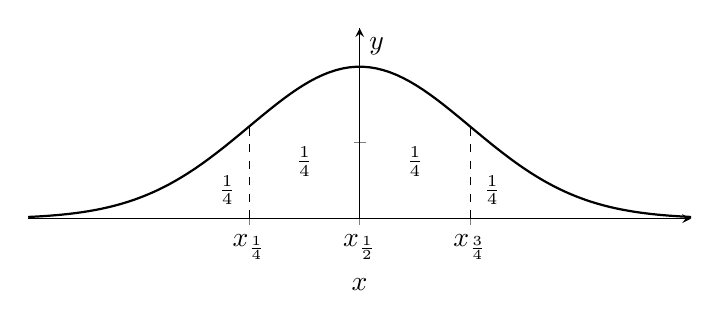
\begin{tikzpicture}

    \definecolor{siva}{rgb}{0.8, 0.8, 0.8}

    \begin{axis}[
        axis lines = left,
        xlabel = $x$,
        ylabel = {$y$},
        domain=-3:3,
        samples=100,
        height=4cm,
        width=10cm,
        xmin=-3, xmax=3,
        ymin=0, ymax=0.5,
        xtick={-1, 0, 1},
        xticklabels={$x_{\frac{1}{4}}$, $x_{\frac{1}{2}}$, $x_{\frac{3}{4}}$},
        yticklabels={},
        axis y line=middle
    ]
    
    \addplot [black, thick] {1/(sqrt(2*pi))*exp(-((x)^2/2)};
    \draw (0,1) -- (0,0);
    \draw[dashed] (-1, 0) -- (-1, 0.242);
    \draw[dashed] (1, 0) -- (1, 0.242);
    
    \node at (-1.2,0.075) {\small $\frac{1}{4}$};
    \node at (-0.5,0.15) {\small $\frac{1}{4}$};
    \node at (0.5,0.15) {\small $\frac{1}{4}$};
    \node at (1.2,0.075) {\small $\frac{1}{4}$};

    \end{axis}
\end{tikzpicture}

\begin{zgled}
    Telesna višina odraslih moških:
    
    \begin{tikzpicture}

        \definecolor{siva}{rgb}{0.8, 0.8, 0.8}

        \begin{axis}[
            axis lines = left,
            xlabel = $x$,
            ylabel = {$y$},
            domain=-3:3,
            samples=100,
            height=4cm,
            width=10cm,
            xmin=-3, xmax=3,
            ymin=0, ymax=0.5,
            xtick={0},
            xticklabels={178},
            yticklabels={}
        ]
        
        \addplot [black, thick] {1/(sqrt(2*pi))*exp(-(x^2/2)};
        \draw[dashed] (0, 0) -- (0, 0.3989);
    
        \end{axis}
    \end{tikzpicture}
\end{zgled}

\n \emph{(Semi)kvartilni razmik} je: 
$$
s=\frac{1}{2}\left(x_{\frac{3}{4}}-x_{\frac{1}{4}}\right)
$$

ki je nadomestek za standardno deviacijo. 

\s

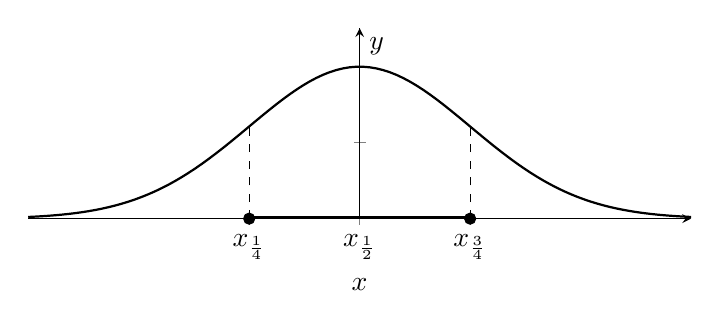
\begin{tikzpicture}

    \definecolor{siva}{rgb}{0.8, 0.8, 0.8}

    \begin{axis}[
        axis lines = left,
        xlabel = $x$,
        ylabel = {$y$},
        domain=-3:3,
        samples=100,
        height=4cm,
        width=10cm,
        xmin=-3, xmax=3,
        ymin=0, ymax=0.5,
        xtick={-1, 0, 1},
        xticklabels={$x_{\frac{1}{4}}$, $x_{\frac{1}{2}}$, $x_{\frac{3}{4}}$},
        yticklabels={},
        axis y line=middle
    ]
    
    \addplot [black, thick] {1/(sqrt(2*pi))*exp(-((x)^2/2)};
    \draw (0,1) -- (0,0);
    \draw[dashed] (-1, 0) -- (-1, 0.242);
    \draw[dashed] (1, 0) -- (1, 0.242);
    \draw[line width=2pt] (-1,0) -- (1,0);
    \addplot[mark=*] coordinates {(-1,0)};
    \addplot[mark=*] coordinates {(1,0)};

    \end{axis}
\end{tikzpicture}

\begin{zgled} ~

    \begin{enumerate}
        \item $X \sim \operatorname{N}(0,1)$:
        $$
        s=\frac{1}{2}\left(x_{\frac{3}{4}}-x_{\frac{1}{4}}\right) = x_{\frac{3}{4}}\approx 0.67
        $$
        \item Cauchyjeva porazdelitev, $p(x)=\frac{1}{\pi\left(1+x^2\right)}$ nima momentov.
        
        Zaradi simetrije velja $x_{\frac{1}{2}}=0$. 
        $$
        \int_0^{x_{\frac{3}{4}}} \frac{1}{\pi\left(1+x^2\right)} \, d x=\frac{1}{4}
        $$

        \begin{tikzpicture}
            \begin{axis}[
                axis lines = left,
                xlabel = $x$,
                ylabel = {$y$},
                domain=-3:3,
                samples=100,
                height=4cm,
                width=10cm,
                xmin=-3, xmax=3,
                ymin=0, ymax=0.5,
                ytick={0.3183},
                xtick={1},
                yticklabels={$\frac{1}{\pi}$},
                xticklabels={$x_{\frac{3}{4}}$},
                enlargelimits=0.05,
                axis y line=middle,
                yticklabel style={xshift=-2cm}
            ]
            
            \addplot [black, thick] {1/(3.1415 * (1 + x^2))};
            \draw[dashed] (0, 0.3183) -- (-1.58, 0.3183);
            \draw[dashed] (1, 0) -- (1, 0.1592);

            \node at (1.2,0.06) {\small $\frac{1}{4}$};
            \node at (0.6,0.1) {\small $\frac{1}{4}$};
    
            \end{axis}
        \end{tikzpicture}
        $$
        \left.\frac{1}{\pi} \operatorname{arctg} x\right|_0 ^{x_{\frac{3}{4}}}=\frac{1}{4} \implies \operatorname{arctg} x_{\frac{3}{4}}=\frac{\pi}{4}
        $$
        Torej je: 
        $$
        x_{\frac{3}{4}}=1=s \quad \text{in} \quad x_{\frac{1}{4}}=-1
        $$
    \end{enumerate}
\end{zgled}

\chapter{Momentno rodovna funkcija}

\n \emph{Momentno rodovna funkcija} slučajne spremenljivke $X$ je: 
$$
M_X(t)=E\left(e^{t  X}\right)
$$

za tiste $t \in \mathbb{R}$ za katere obstaja matematično upanje, t.j.: $E\left(e^{t X}\right)<\infty$.

\n Kadar ima $X$ vrednosti v $\mathbb{N} \cup \{0\}$, je: 
$$
M_X(t)=E\left(\left(e^t\right)^X\right)=G_X\left(e^t\right)
$$

torej, gre za posplošitev rodovne funkcije. 

\n Če je $X$ zvezno porazdeljena z gostoto $p(x)$, je: 
$$
M_X(t)=\int_{-\infty}^{\infty} e^{t  x} \, p(x) \, d x
$$

kar je \emph{Laplaceova transformacija} funkcije $p$. 

\begin{zgled}
    $X \sim \operatorname{N}(0,1)$:
    $$
    \begin{aligned}
        M_X(t)&=\frac{1}{\sqrt{2 \pi}} \int_{-\infty}^{\infty} e^{t x} \, e^{-\frac{x^2}{2}} \,d x \\
        &=e^{\frac{t^2}{2}} \underbrace{\frac{1}{\sqrt{2} \pi} \int_{-\infty}^{\infty} e^{-\frac{1}{2}(x-t)^2} \, d x}_{\text {gostota za } N(t, 1)} \\
        &=e^{\frac{t^2}{2}}
    \end{aligned}
    $$
\end{zgled}

\begin{izrek}
    Naj obstaja $\delta > 0$, da je $M_X(t)<\infty$, za vse $t \in(-\delta, \delta)$. Potem je porazdelitev $X$ natanko določena z $M_X$, vsi začetni momenti obstajajo: 
    $$
    \begin{aligned}
        & z_k=E\left(X^k\right)=M_X^{(k)}(0) \quad \text {za vse} \quad  k \in \mathbb{N} & \\
        & M_X(t)=\sum_{k=0}^{\infty} \frac{z_k}{k !} t^k \quad \text{za vse} \quad {t \in(-\delta, \delta)} &
    \end{aligned}
    $$
\end{izrek}

\begin{proof}(skica)
    $$
    \begin{aligned}
        M_X(t)&=E\left(e^{t X}\right) \\
        &=E\left(\sum_{k=0}^{\infty} \frac{X^k}{k !}  t^k\right) \\
        &=\sum_{k=0}^{\infty} \frac{E\left(X^k\right)}{k !} t^k \\
        &=\sum_{k=0}^{\infty} \frac{z_k}{k !} t^k
    \end{aligned}
    $$
\end{proof}

\begin{trditev}
    $$
    M_{a X+b}(t)=e^{b t} \, M_X(a t) \quad \text{za} \quad a \neq 0, b \in \mathbb{R}
    $$
\end{trditev}

\begin{proof}
    $$
    \begin{aligned}
        M_{a X+b}(t)&=E\left(e^{t(a X+b)}\right) \\
        &=E\left(e^{(a t) X} \, e^{b t}\right) \\
        &=e^{b t} \, M_X(a t)
    \end{aligned}
    $$
\end{proof}

\begin{trditev}
    Za $X \sim \operatorname{N}(\mu, \sigma)$ velja: 
    $$
    M_X(t)=e^{\mu t+\frac{\sigma^2 t^2}{2}}
    $$
\end{trditev}

\begin{proof}
    Definiramo: $U:=\frac{X-\mu}{\sigma} \sim N(0,1)$, zato $X=\sigma U+\mu$:
    $$
    \begin{aligned}
        M_X(t)&=M_{\sigma U+\mu}(t) \\
        &=e^{\mu t} \, M_U(\sigma\, t) \\
        &=e^{\mu t} \, e^{\frac{\sigma^2 t^2}{2}} \\
        &=e^{\mu t+\frac{\sigma^2 t^2}{2}}
    \end{aligned}
    $$
\end{proof}

\begin{izrek}
    Če sta $X$ in $Y$ neodvisni slučajni spremenljivki, potem je:
    $$
    M_{X+Y}(t)=M_X(t) \, M_Y(t)
    $$
\end{izrek}

\begin{proof}
    \begin{align*}
        M_{X+Y}(t)&=E\left(e^{t (X+Y)}\right) \\
        &=E\left(e^{t X} \, e^{t  Y}\right) \tag{$\star$} \\
        &=E\left(e^{t X}\right) E\left(e^{tY}\right) \\
        &=M_X(t) \, M_Y(t)
    \end{align*}

    Kjer smo v $(\star)$ vrstici upoštevali neodvisnost.
\end{proof}

\begin{trditev}
    Imejmo $X \sim \operatorname{N}(\mu_X, \sigma_X)$ in $Y \sim \operatorname{N}(\mu_Y, \sigma_Y)$ neodvisni slučajne spremenljivki. Potem je: 
    $$
    X+Y \sim N\left(\mu_X+\mu_Y, \sqrt{\sigma_X^2+\sigma_Y^2}\right)
    $$
\end{trditev}

\begin{opomba}
    \begin{flalign*}
        &\qquad E(X+Y)=E(X)+E(Y)=\mu_X+\mu_Y & \\
        &\qquad D(X+Y)=D(X)+D(Y)=\sigma_X^2+\sigma_Y^2 & 
    \end{flalign*}
\end{opomba}

\begin{proof}
    $$
    \begin{aligned}
        M_{X+Y}(t)&=M_X(t) \, M_Y(t) \\
        &=e^{\mu_X t+\frac{\sigma_X^2 t^2}{2}} \, e^{\mu_Y t+\frac{\sigma_Y^2 t^2}{2}} \\
        &=e^{\left(\mu_X+\mu_Y\right) t+\frac{\sigma_X^2+\sigma_Y^2}{2} t^2} 
    \end{aligned}
    $$

    od koder zaradi enoličnosti sledi:
    $$
    X+Y \sim \operatorname{N}\left(\mu_X\mu_Y, \sqrt{\sigma_X^2+\sigma_Y^2}\right)
    $$
\end{proof}

\begin{zgled}
    Za $\operatorname{N}(0,1)$ izračunajmo vse momente:
    $$
    \begin{aligned}
        M_X(t)&=e^{\frac{t^2}{2}} \\
        &=\sum_{k=0}^{\infty} \frac{1}{k !}\left(\frac{t^2}{2}\right)^k \\
        &=\sum_{k=0}^{\infty} \frac{t^{2 k}}{2^k \, k !}
    \end{aligned}
    $$
    $\qquad \implies z_{2 k+1}=0 \quad \forall k$
    
    Po drugi strani pa je:
    $$
    M_X(t)=\sum_{k=0}^{\infty} \frac{z_k}{k !}  t^k
    $$

    Po primerjavi koeficientov dobimo: 
    $$
    \frac{z_{2 k}}{(2 k) !}=\frac{1}{2^k \, k !}
    $$

    Od tod sledi: 
    $$
    z_{2 k}=\frac{(2 k) !}{2^k \, k !}=\frac{1 \cdot 2 \cdot 3\cdots  2 k}{2 \cdot 4 \cdot 6 \cdots 2 k }=1 \cdot 3 \cdot 5 \cdot 7 \cdots (2 k-1)=(2 k-1) ! !
    $$
\end{zgled}

\end{document}